\documentclass[
  a4paper,
  upppercaseChapter,
  normalTOC,
  noIndentAnAp,
  fancyPlainHeader,
  samePageChapter
]{academix/academix}

% ------------------------------------------------------------------
% HYPERLINKS AND PDF CONFIGURATION
% ------------------------------------------------------------------

% Enables hyperlinks and defines their appearance
\usepackage[
  bookmarks,
  colorlinks,
  citecolor=black,
  urlcolor=blue,
  linkcolor=black,
  pdfpagemode=UseNone
]{hyperref}

% ------------------------------------------------------------------
% MATHEMATICS SUPPORT
% ------------------------------------------------------------------

% Math support for advanced typesetting (equations, theorems, symbols):
% - amsmath: Advanced math typesetting
% - amsfonts: Extra math fonts
% - amssymb: Additional math symbols
% - amsthm: Theorem-like environments (theorems, lemmas, etc.)
\usepackage{amsmath, amsfonts, amssymb, amsthm}

% Use Times-like font (newtxtext and newtxmath) for both text and math symbols
\usepackage{newtxtext, newtxmath}

% Define theorems with consistent formatting
\newtheorem{theorem}{Theorem}{\bfseries}{\itshape}
\newtheorem{lemma}{Lemma}{\bfseries}{\itshape}
\newtheorem{definition}{Definition}{\bfseries}{\itshape}
\newtheorem{corollary}{Corollary}{\bfseries}{\itshape}
\newtheorem{assumption}{Assumption}{\bfseries}{\itshape}
\newtheorem{proposition}{Proposition}{\bfseries}{\itshape}
\newtheorem{remark}{Remark}{\bfseries}{\itshape}

% Define a custom theorem style for examples
\newtheoremstyle{example}
  {1em}        % Space above
  {1em}        % Space below
  {}           % Body font
  {}           % Indent amount
  {\bfseries}  % Theorem head font
  {:}          % Punctuation after theorem head
  {0.5em}      % Space after theorem head
  {\thmname{#1}\thmnumber{ #2}\thmnote{ #3}} % Theorem head specification

% Apply the custom style to examples
\theoremstyle{example}
\newtheorem{example}{Example}

% ------------------------------------------------------------------
% FONT AND ENCODING SETTINGS
% ------------------------------------------------------------------

% Set font encoding to T1 for proper handling of special characters (accents, etc.)
\usepackage[T1]{fontenc}

% Set Helvetica as the default sans-serif font (similar to Arial)
% - \sfdefault: Use sans-serif fonts for the entire document
\usepackage{helvet}
\renewcommand{\familydefault}{\sfdefault}

% ------------------------------------------------------------------
% LANGUAGE SUPPORT
% ------------------------------------------------------------------

% Language support for English (proper hyphenation and text rules)
\usepackage[english]{babel}

% ------------------------------------------------------------------
% CITATION MANAGEMENT
% ------------------------------------------------------------------

% ABNT Style
% Citation management using ABNT (Brazilian Technical Standards):
% - alf: Use the alphanumeric citation style (author-date format).
% - abnt-repeated-author-omit=yes: Omit repeated authors in the bibliography, replacing them with a dash (---).
% - abnt-title-command=yes: Enable \citeauthor and \citetitle commands for citing only the author or the title.
% - abnt-emphasize=bf: Emphasize the author's name in bold in citations.
% \usepackage[
%   alf,
%   abnt-repeated-author-omit=yes,
%   abnt-title-command=yes,
%   abnt-emphasize=bf
% ]{abntex2cite}

% APA Style
\usepackage{cite}
\bibliographystyle{apalike}

% Proper formatting and line breaking for URLs
\usepackage{url}

% ------------------------------------------------------------------
% TABLES
% ------------------------------------------------------------------

% Professional-quality tables with enhanced rules and spacing
\usepackage{booktabs}

% Support for large tables that can span multiple pages
% (not compatible with two column)
\usepackage{longtable}

% Combines longtable with tabularx for dynamic column width adjustment in large tables
\usepackage{ltxtable}

% ------------------------------------------------------------------
% FLOATS AND GRAPHICS
% ------------------------------------------------------------------

% Enhanced control over float objects (figures, tables):
% - Allows precise placement of floating objects using the [H] option
\usepackage{float}

% Graphics and images support:
% - pdftex: Use PDFLaTeX engine for image handling
% - graphicspath: Set the directory for images to 'figures/'
% - DeclareGraphicsExtensions: Define preferred image file formats (PDF, JPEG, PNG, JPG)
\usepackage[pdftex]{graphicx}
\graphicspath{{figures/}}
\DeclareGraphicsExtensions{.pdf,.jpeg,.png,.jpg}

% Insert external PDF documents into the LaTeX document
\usepackage{pdfpages}

% ------------------------------------------------------------------
% MISCELLANEOUS
% ------------------------------------------------------------------
\renewcommand{\customChapterMark}[1]{\markboth{#1}{}}
\renewcommand{\customSectionMark}[1]{\markright{#1}{}}
\newcommand{\source}[1]{\\Source: {#1}}

\customAuthor{John Doe}
\customTitle{Title}
\location{Gotham}
\customDate{2024}

\advisor{Professor John Doe}
\minipageText{Thesis submitted for the degree of Master of Science to the School of Engineering.}
\concentrationArea{Systems Engineering}

\dedication{To my family}

\sloppy

\begin{document}

% -------------
% External part
% -------------
\coverPage


% -------------
% Internal part
% -------------

% Pre-textual elements
\pagenumbering{roman}
\backCover
\dedicationPage
\begin{acknowledgement}
I thank all the people who...
\end{acknowledgement}

\begin{abstract}

    In this work we study the...

    \vspace{1\baselineskip}

    \textbf{Keywords:} Stochastic control. Linear systems. Optimal control. Maximum variance. Portfolio optimization.

\end{abstract}

\begin{secondAbstract}

    In this work, we study the...

    \vspace{1\baselineskip}

    \textbf{Keywords:} Stochastic control. Linear systems. Optimal control. Maximum variance. Portfolio optimization.

\end{secondAbstract}

\listoffigures
\listoftables
\begin{listofabbreviations}{1000}
    \item [USP] Universidade de São Paulo
    \item [IPP] Institut Polytechnique de Paris
\end{listofabbreviations}

\begin{listofsymbols}{1000}
	\item [$\Delta(h)$] Assinatura di\' adica
\end{listofsymbols}

\tableofcontents

% Textual elements
\chapter{Introduction} \label{chap:intro}

Here you should give the context, justifications...

Do yourself a favor and follow the structure guidelines in the file \texttt{Research struc\-ture guidelines.md}. It should make your life easier.

In this template I will leave examples on how to cite, reference chapters, tables, figures, use math symbols along the text, write equations, label them for further referencing, use cases in equations, write tables, include figures, use special math formatting and symbols, use proof environments for theorems, matrix environments, etc. Remember to build the main file \texttt{thesis\_main.tex} to visualize the updated pdf.

Example of how to reference a chapter: This dissertation is structured in several chapters. In Chapter \ref{chap:lit}, we present a detailed review of the literature, highlighting key contributions in the field. For example, the work by Doe and Smith \cite{doe0000} provides a foundational analysis on this topic, which serves as a basis for the methodology discussed in Chapter \ref{chap:method}.



\pagenumbering{arabic}
\chapter{Literature review} \label{chap:lit}


\chapter{Methodology} \label{chap:method}

Introduction here...

\section{Notation and definitions} \label{notation}

Throughout this work the $n$-dimensional real Euclidean space will be denoted by $\mathbb{R}^{n}$ and the linear space of all $m \times n$ real matrices by $\mathbb{B}(\mathbb{R}^{n},\mathbb{R}^{m})$,  with $\mathbb{B} (\mathbb{R}^{n})$\,$:=$\,$\mathbb{B}(\mathbb{R}^{n},\mathbb{R}^{n})$.

We denote by $\mathbb{H}^{n,m}$ the linear space made up of all $N$-sequences of real matrices $V$\,$=$\,$(V_{1},\dotsc,V_{N})$ with $V_{i}$\,$\in$\, $\mathbb{B}(\mathbb{R}^{n},\mathbb{R}^{m})$, for $i$\,$=$\,$1,\dotsc,N$ and, for simplicity, set $\mathbb{H}^{n}$\,$:=$\,$\mathbb{H}^{n,n}$.

We say that $V$\,$=$\,$(V_{1},\dotsc,V_{N})$\,$\in$\,$\mathbb{H}^{n+}$ if $V$\, $\in$\,$\mathbb{H}^{n}$ and $V_{i}$\,$\geqslant$\,$0$, for each $i$\,$=$\,$1,\dotsc,N$. The space of all bounded linear operators from $\mathbb{H}^{n}$ to $\mathbb{H}^{m}$ will be represented by $\mathbb{B}(\mathbb{H}^{n}, \mathbb{H}^{m})$ and, in particular, $\mathbb{B}(\mathbb{H}^{n})$\,$:=$\, $\mathbb{B}(\mathbb{H}^{n},\mathbb{H}^{n})$.

We use the standard notation for $tr(A)$, $A'$, and $A^{\dagger}$ to represent the trace, transpose, and Moore-Penrose inverse of $A$ respectively.

The Kronecker product between two matrices $A$ and $B$ will be denoted by $A$\, $\otimes$\,$B$, and the identity matrix (of appropriate dimension from the context) will be represented by $I$.

For a sequence of $n$-dimensional square matrices $A(0),\dotsc,A(t)$, we use the notation:

\begin{flalign*}
    \prod_{l=s}^{t}A(l) =
    \begin{cases}
        A(t)\dotsm A(s) \text{ for } t \geqslant s, \\
        I \text{ for } t<s.
    \end{cases}
\end{flalign*}

For a set $S$ we define $1_{s}$ as the usual indicator function, that is,

\begin{flalign*}
    1_{s}(\omega) =
    \begin{cases}
        1  \text{ if } \omega \in S, \\
        0 \text{ otherwise}.
    \end{cases}
\end{flalign*}

\section{The linear system with Markov jumps and multiplicative noises} \label{MJLS}

We consider the following linear system with multiplicative noises and Mar\-kov jumps on a probabilistic space $(\Omega,\textbf{P},\mathcal{F})$ for $k=0, \cdots, T-1$ and $t=1, \cdots, T$:

\begin{flalign} \label{eq:system}
    x(k+1) = {} & \left[ \bar{A}_{\theta(k)}(k)\;+\;\sum^{\varepsilon^{x}}_{s=1} \tilde{A}_{\theta(k),s}(k)w^{x}_{s}(k)\right]x(k)+\left[\bar{B}_{\theta(k)}(k)\;+\;\sum^{\varepsilon^{u}}_{s=1} \tilde{B}_{\theta(k),s}(k)w^{u}_{s}(k)\right]u(k), & \nonumber \\
    x(0) = {} & x_{0}, \; \theta(0) = \theta_{0},     &
\end{flalign}

\begin{flalign} \label{eq:output}
     & y(t)=L_{\theta(t)}(t)x(t), &
\end{flalign}
where $L_{\theta(t)}(t) \in \mathbb{H}^{1,n}$.

Here, $s$  refers to the $s^{th}$ column vector  and $\theta(k)$ denotes the
operation modes of a time-varying Markov chain taking values in \{1,$\dotsc$,N\} with transition probability matrix $\mathbb{P}(k)$ = $[\textit{p}_\textit{ij}(k)]$.

We define $\mathcal{F}_{\tau}$ as the $\sigma$-field generated by
$\{(\theta(s),x(s));s$\,$=$\ $0,\dotsc,\tau \}$, $\mathcal{F}_{k}$ - measurable
for each $k = \tau, \cdots, T-1$ and write $\mathbb{U}(\tau)$ $=$
$\{u_{\tau}$\,$=$\ $( u(\tau),\dotsc,u(T-1) )\}$, where $u(k)$ is an $m$-dimensional
random vector with finite second moments.

Without loss of generality, we assume that $\varepsilon$\,$=$\,
$\varepsilon^{x}$\,$=$\,$\varepsilon^{u}$, and the superscript $^{u}$ will
indicate that the control law $u$ is being applied to (\ref{eq:system}) and
(\ref{eq:output}).

We have that, for each $s$ $=$ $1,\dotsc,\varepsilon$ and $k = 0,1,\cdots, T$,
\begin{flalign*}
    & \bar{A}(k) = (\bar{A}_{1}(k),\dotsc,\bar{A}_{N}(k)) \in \mathbb{H}^{n},                 \\
    & \tilde{A}_{s}(k) = (\tilde{A}_{s,1}(k), \dotsc,\tilde{A}_{s,N}(k)) \in 	\mathbb{H}^{n}, \\
    & \bar{B}(k) = (\bar{B}_{1}(k), \dotsc, \bar{B}_{N}(k)) \in \mathbb{H}^{m,n},             \\
    & \tilde{B}_{s}(k) = (\tilde{B}_{s,1}(k),\dotsc,\tilde{B}_{s,N}(k)) \in \mathbb{H}^{m,n}.
\end{flalign*}

The multiplicative noises
$\{w_{s}^{x}(k)$; $s$ $=$ $1,\dotsc,\varepsilon^{x}$, $k$ $=$ $0,1,\dotsc,T$
$-$ $1\}$ and
$\{w_{s}^{u}(k)$; $s$ $=$ $1,\dotsc,\varepsilon^{u}$, $k$ $=$ $0,1,\dotsc,T$
$-$ $1\}$
are both zero-mean random variables with variance equal to 1 and also independent of the Markov chain $\{\theta(k)\}$.
The independence among their elements are set as $E[w^{x}_{i}(k)w^{x}_{j}(l)]=0$ and $E[w^{u}_{i}(k)w^{u}_{j}(l)]=0$, $\forall$ $k=l$ and $i\neq j$, or $\forall$ $k\neq l$ and $\forall$\,$i,j$.

The mutual correlation between $w^{x}_{s1}(k)$ and $w^{u}_{s2}(k)$ is denoted
by $E[w^{x}_{s1}(k)w^{u}_{s2}(k)]=\rho_{s1,s2}(k)$.

The initial conditions $\theta_{0}$ and $x_{0}$ are assumed to be independent
of $\{w_{s}^{x}(k)\}$ and $\{w_{s}^{u}(k)\}$, with $x_{0}$ an $n$-dimensional
random vector with finite second moments.

We also set the following expected values regarding the state variable.
\begin{flalign*}
     & \mu_{i}(0) = E(x_{0}1_{\{\theta_{0}=i\}}),                           \\
     & \mu(0) = [\mu_{1}(0)'\;\dotsc \; \mu_{N}(0)']\ \in \mathbb{H}^{n,1}, \\
     & Q_{i}(0) = E(x_{0}x_{0}'1_{\{\theta_{0}=i\}}),  \text{ and }         \\
     & Q(0)= [Q_{1}(0)\;\dotsc\;Q_{N}(0)] \in \mathbb{H}^{n+}.
\end{flalign*}

\section{The constrained problem formulation, $PC(\nu,\beta,\alpha)$} \label{obj_formul}

Our goal in this work is to find the optimal control policy, $u$, to the constrained problem denoted by $PC(\nu,\beta,\alpha)$ and defined as:

\begin{flalign} \label{PC3}
     & PC(\nu,\beta,\alpha): \max_{u \in \mathbb{U}} \sum_{t=1}^{T} \biggl[
    \beta(t)E\big[ y^{u}(t) \big] \biggr],  \nonumber                                          \\
     & \text{subject to:} \quad \sum_{t=1}^{T} \nu(t)Var\big[ y^{u}(t) \big] \leqslant \alpha,
\end{flalign}

where
$ \beta = [\beta(1) \cdots \beta(T)]', \; \beta(t) \geqslant 0$, is the input
parameter associated with system's output, $\nu=[\nu(1) \cdots \nu(T) ]',\; \nu(t) \geqslant 0$, is the input parameter associated with the variance of the system's output,
and $\alpha \geqslant 0$ is the maximum total weighted variance of the system's output.

In this problem, the parameters $\beta$, $\nu$, and $\alpha$ are provided by the user and can be seen as risk aversion coefficients reflecting a trade-off preference between the expected output and the associated risk (variance) level.

It is worth to mention that there is no formula to compute these parameters and they depend on the user's sensibility and capacity to "translate" risk aversion preferences between the expected output and the associated variance level into coefficients we can use in our model.

To assist someone on the task of computing these coefficients, we provide in Section \ref{s2} and Appendix \ref{app:A} a detailed sensitivity analysis regarding $\nu$ and $\beta$ for a certain level of $\alpha$.
However, just to illustrate the effects of these coefficients, we will also provide the following rather simple example.

Let's assume that $y^u(t)$ represents the absolute value, in monetary terms, of a portfolio of risk investment securities, where $u$ corresponds to the optimal allocation of the assets over the period of time $T$.
For simplicity, we will only consider a three-week period, $T=3$, an initial portfolio's value  of $\$1,000$, and that the investor wishes to limit the total variance of the portfolio's value to $\$30$ over the three-week period.

    Let's also consider, in our example, that the investor is less averse to fluctuations in the expected value of the portfolio in the first week than in the the last two weeks by a multiple of $1.4$.
    In the same way, consider that he/she is more averse to fluctuations in the variance in the second week  than in the first or third week by a multiple of $1.7$.


    In this way, the investor could define $\alpha = 30$,  $\beta = [1.4\; 1\; 1]$, and $\nu = [1 \;1.7\; 1]$ in order to take into consideration the aversion towards risks as stated in the specific example above and to find an optimal allocation using $PC(\nu,\beta,\alpha)$.

    Note that the relative weights between the elements of $\nu$ and $\beta$ are also relevant.
    %
    However, as we will see in Chapter \ref{chap:res}, when we impose a total weighted variance $\alpha$, there must be an adjustment between these relative weights in order to accommodate the new restriction on the variance. % with a correspondent new proper level
    %
    Intuitively, if we want to fix a lower total variance it could only be achieved if we accept lower returns and conversely, if we want to fix a higher total variance it could only be achieved if we "accept" higher returns.

    Notwithstanding, lower or higher returns can be set by adjusting the coefficients of $\beta$ as we will see when we present the solution of $PC(\nu,\beta,\alpha)$ in Chapter \ref{chap:res}.
    Thereby, our objective can be rephrased to finding the exactly expected level of the output that leads to the desired total weighted variance restriction, $\alpha$, which in turn can be achieved by properly adjusting $\beta$.

    \section{The unconstrained problem formulation, $PU(\nu,\xi)$} \label{uproblem}

    The mean-variance cost function is defined as, for all $u \in \mathbb{U}$,

    \begin{flalign} \label{costU}
        \mathcal{C}(u) := \sum_{t=1}^{T} \biggl[ \nu(t)Var\big[ y^{u}(t) \big]
            -\xi(t)E\big[ y^{u}(t) \big] \biggr],
    \end{flalign}
    where $\xi=[\xi(1) \cdots \xi(T) ]',\;\xi(t) \geqslant 0$, is the input parameter associated with the system's output and $\nu(t) \geqslant 0$ is the input parameter as defined in problem (\ref{PC3}).
    In the same way as in problem (\ref{PC3}), the input parameters $\xi$ and $\nu$ can be seen as risk aversion coefficients reflecting a trade-off preference between the expected output and the associated risk (variance) level, respectively.

    The optimal control strategy of problem $PC(\nu,\beta,\alpha)$ will be obtained through the solution of the mean-variance unconstrained problem denoted by $PU(\nu,\xi)$ and defined as:

    \begin{flalign} \label{PU}
        PU(\nu,\xi):\; \min_{u \in \mathbb{U}} \mathcal{C}(u).
    \end{flalign}

    Since problem $PU(\nu,\xi)$ involves a nonlinear function of an expectation
    term in $Var\big[ y^{u}(t) \big] = E\big[ y^{u}(t)^{2} \big] - E\big[  y^{u}(t)
    \big]^{2}$, it cannot be directly solved by dynamic programming and the
    following tractable auxiliary problem is solved instead.
    %
    \begin{flalign} \label{AP}
        A(\nu, \lambda):=\; \min_{ u \in \mathbb{U} } E \Biggl\{ \sum_{t=1}^{T}\biggl[ \nu(t)y^{u}
        (t)^{2} - \lambda(t)y^{u}(t) \biggr] \Biggr\} ,
    \end{flalign}
    %
    where $\lambda=[\lambda(1) \cdots \lambda(T) ]',\; \lambda(t) \geqslant 0$.

    Thus, the solution of problem (\ref{AP}) leads to the same solution of problem (\ref{PU}) and the reader is referred to \cite{doe0000} for more detailed information and proofs.

    \section{Mathematical operators} \label{operators}

    For $k$\,$=$\,$0,\dotsc,T-1$, $X$\,$\in$\,$\mathbb{H}^{n}$, and $i$\,$=$\,$1,\dotsc,N$ the following operators will be useful in the sequel to obtain the optimal control strategy of Problem (\ref{PU}) through the solution of Problem (\ref{AP}). \\ $\bullet$ \textbf{Expected value operator,} $\mathcal{E}(k,\cdot)$: \\ $\mathcal{E}(k,\cdot) \in \mathbb{B}(\mathbb{H}^{n}):$

    \begin{flalign} \label{eq:pv}
        \mathcal{E}_{i}(k,X)=\sum_{j=1}^{N}p_{ij}(k)X_{j}.
    \end{flalign}

$\bullet$ \textbf{Auxiliary operators}, $\mathcal{A}(k,\cdot)$, $\mathcal{G}(k,\cdot)$, and $\mathcal{R}(k,\cdot)$: \\
$\mathcal{A}(k,\cdot) \in \mathbb{B}(\mathbb{H}^{n}):$
    \begin{flalign} \label{eq:Ai}
        \mathcal{A}_{i}
        (k,X)=\bar{A}_{i}(k)'\mathcal{E}_{i}(k,X)\bar{A}_{i}(k)
        +\sum_{s=1}^{\varepsilon}\tilde{A}_{i,s}(k)'\mathcal{E}_{i}
        (k,X)\tilde{A}_{i,s}(k).
    \end{flalign}
    %
$\mathcal{G}(k,\cdot) \in \mathbb{B}(\mathbb{H}^{n,1},\mathbb{H}^{n,m}):$
    \begin{flalign} \label{eq:Gi}
        \mathcal{G}_{i}(k,X)= \Biggl[ \bar{A}_{i}(k)'
            \mathcal{E}_{i}(k,X) \bar{B}_{i}(k) + \sum_{s1=1}^{\varepsilon}
            \sum_{s2=1}^{\varepsilon} \rho_{s1,s2}(k) \tilde{A}_{i,s1}(k)'
            \mathcal{E}_{i}(k,X) \tilde{B}_{i,s2}(k)\Biggr]'.
    \end{flalign}
$\mathcal{R}(k,\cdot)  \in \mathbb{B}(\mathbb{H}^{n},\mathbb{H}^{m}):$
    \begin{flalign} \label{eq:Ri}
        \mathcal{R}_{i}(k,X)=\bar{B}_{i}(k)'\mathcal{E}_{i}(k,X)
        \bar{B}_{i}(k)+\sum_{s=1}^{\varepsilon}\tilde{B}_{i,s}(k)'\mathcal{E}_{i}
        (k,X)\tilde{B}_{i,s}(k).
    \end{flalign}
$\bullet$ \textbf{Operator associated with the feedback gain of the optimal control law}, $\mathcal{K}(k,\cdot)$:
    \begin{flalign} \label{eq:Ki}\
        \mathcal{K}_{i}(k,X)=\mathcal{R}_{i}(k,X)^{\dagger}\mathcal{G}_{i}(k,X),
        \text{ and } \nonumber \\ K_{i}(k)={}&\mathcal{K}_{i}(k,P(k+1)).
    \end{flalign}
$\bullet$ \textbf{Operator associated with the generalized coupled Riccati difference equation}, $\mathcal{P}(k,\cdot)$:
    \begin{flalign} \label{eq:Pi}
        \mathcal{P}_{i}(k,X)=\mathcal{A}_{i}(k,X)-\mathcal{G}_{i}(k,X)'
        \mathcal{R}_{i}(k,X)^{\dagger}\mathcal{G}_{i}(k,X)
        +\nu(k)L_{i}(k)'L_{i}(k), \text{ and } \nonumber \\
        P_{i}(k) = \mathcal{P}_{i}(k,P(k+1)).
    \end{flalign}
$\bullet$ \textbf{Operators related to the presence of the linear term in problem (\ref{AP})}, $\mathcal{V}(k,\cdot,\cdot)$ and $\mathcal{H}(k,\cdot)$: \\
$\mathcal{V}(k,\cdot,\cdot) \in \mathbb{B}(\mathbb{H}^{n,1},\mathbb{H}^{n,m}):$
    \begin{flalign} \label{eq:Vi}
        \mathcal{V}_{i}(k,X,V)=\mathcal{E}_{i}(k,V) \bigl[ \bar{A}_{i}(k)
            -\bar{B}_{i}(k)\mathcal{K}_{i}(k,X) \bigr] + \lambda(k)L_{i}(k),
        \text{ and} \nonumber \\
        V_{i}(k)= \mathcal{V}_{i}(k,P(k+1),V(k+1)).
    \end{flalign}
    %
$\mathcal{H}(k,\cdot) \in \mathbb{B}(\mathbb{H}^{n,1},\mathbb{H}^{n,m}):$
    \begin{flalign} \label{eq:Hfi}
        \mathcal{H}_{i}(k,V)
        =\bar{B}_{i}(k)'\mathcal{E}_{i}(k,V)', \text{ and} \nonumber \\
        H_{i}(k)= \mathcal{H}_{i}(k,V(k+1)).
    \end{flalign}

    The following definitions are used to obtain a simplified formula for some parameters that will be used in the sequel.
    \begin{flalign} \label{eq:gamma}
        \Gamma =
        \left[
            \begin{matrix}
                \nu(1) & \cdots & 0      \\
                \vdots & \ddots & \vdots \\
                0      & \cdots & \nu(T)
            \end{matrix}
            \right].
    \end{flalign}

    \begin{flalign} \label{eq:Av}
        A_{i}^{cl}(k) = \bar{A}_{i}(k)-\bar{B}_{i}(k)K_{i}(k),  \nonumber \\
        \mathbb{A}(k) =
        \left[
            \begin{matrix}
                p_{11}(k)A_{1}^{cl}(k) & \cdots & p_{N1}(k)A_{N}^{cl}(k) \\
                \vdots                 & \ddots & \vdots                 \\
                p_{1N}(k)A_{1}^{cl}(k) & \cdots & p_{NN}(k)A_{N}^{cl}(k)
            \end{matrix}
            \right].
    \end{flalign}

    \begin{flalign} \label{eq:Dv}
        \mathbb{Q}_{i}(k) = \pi_{i}(k)\bar{B}_{i}(k)\mathcal{R}_{i}
        (k,P(k+1))^{\dagger}\bar{B}_{i}(k)' \geqslant 0,  \nonumber \\
        \mathbb{D}(k) =
        \left[
            \begin{matrix}
                \mathbb{Q}_{1}(k) & \cdots & 0                 \\
                \vdots            & \ddots & \vdots            \\
                0                 & \cdots & \mathbb{Q}_{N}(k)
            \end{matrix}
            \right] \geqslant 0 .
    \end{flalign}

    \begin{flalign} \label{eq:Zv}
        \mathbb{Z}(k) = \left[ \mathbb{P}(k)\otimes I \right]'\mathbb{D}(k)
        \left[ \mathbb{P}(k)\otimes I \right] \geqslant 0.
    \end{flalign}

    \begin{flalign} \label{eq:Lv}
        \mathbb{L}(k) = \left[ L_{1}(k) \cdots L_{N}(k) \right].
    \end{flalign}

    \begin{flalign} \label{eq:a}
        a(t) = \mathbb{L}(t)\left[ \prod_{l=0}^{t-1}\mathbb{A}(l) \right]
        \mu(0),\; t=1,\dotsc,T,  \nonumber \\
        a = [a(1) \cdots a(T) ]'.
    \end{flalign}

    Finally, for $ t=1,\dotsc,T$ and $1 \leqslant s \leqslant t$:
    \begin{flalign} \label{eq:Bt}
        g(t,s) =  \mathbb{L}(t)\left[ \prod_{l=s}^{t-1}\mathbb{A}(l) \right]
        \mathbb{Z}(s-1)^{\frac{1}{2}},  \nonumber                         \\
        b(t,s) = \frac{1}{2}\sum_{l=0}^{s-1}g(t,l+1)g(s,l+1)',  \nonumber \\
        \tilde{b}(i,j) =
        \begin{cases}
            b(i,j) \qquad i \geqslant j \\
            b(j,i) \qquad i < j
        \end{cases}, \nonumber                                       \\
        \tilde{\mathbb{B}} =
        \left[
            \begin{matrix}
                \tilde{b}(1,1) & \cdots & \tilde{b}(1,T) \\
                \vdots         & \ddots & \vdots         \\
                \tilde{b}(T,1) & \cdots & \tilde{b}(T,T)
            \end{matrix}
            \right].
    \end{flalign}

    % ****************************************************************************
    % ******************	PREVIOUS RESULTS section
    % ****************************************************************************
    %
    \section{Previous results} \label{pResults}

    The following results represent the minimum previous knowledge we need to solve problem $PC(\nu,\beta,\alpha)$ using the optimal control law of problem $PU(\nu,\xi)$.

    We basically set the conditions and explicit formulas for the optimal control strategy of problem $PU(\nu,\xi)$ and formulas for the expected system's output and total weighted variance.
    Once more, the reader is referred to \cite{doe0000} for further details and proofs.

    Assumption \ref{aH} and Proposition \ref{p:aH} establish the conditions we need in order to
    state that the solution of the auxiliary problem $A(\nu, \lambda)$ will also be the solution of problem $PU(\nu,\xi)$.

    Theorem \ref{t:c_law} provides the optimal control law of $PU(\nu,\xi)$, which depends on $\lambda$ as one can see from Equations  (\ref{eq:Vi}) and (\ref{eq:Hfi}), while Theorem \ref{t:lambda} establishes the identity between the parameter $\lambda$ and the input parameter $\xi$.

    Proposition \ref{p:SVar} gives an explicit formula for the expected value of the output and its total weighted variance when the optimal control policy (\ref{u_k}) is applied.

    \begin{assumption} \label{aH}
        For each $i=1, \dotsc, N \text{ and } k=0, \dotsc, T-1$, we have that
        $H_{i}(k) \in Im(\mathcal{R}_{i}(k,P(k+1)))$.
    \end{assumption}

    \begin{proposition} \label{p:aH}
        If Assumption \ref{aH} holds then
        $H_{i}(k) \in Im(\mathcal{R}_{i}(k,P(k+1)))$
        is satisfied for any $\lambda \in \mathbb{R}^{T}$.
    \end{proposition}

    \begin{proof}
        See Proposition 5 in \cite{doe0000}.
    \end{proof}

    \begin{theorem} \label{t:c_law}
        If Proposition \ref{p:aH} holds then an optimal control strategy for problem $PU(\nu,\xi)$ is achieved by
        \begin{flalign} \label{u_k}
            u(k) = -\mathcal{R}_{\theta(k)}(k,P(k+1))^{\dagger}
            \Bigl[ \mathcal{G}_{\theta(k)}(k,P(k+1))x(k) -
            \frac{1}{2}\mathcal{H}_{\theta(k)}(k,V(k+1)) \Bigr].
        \end{flalign}
    \end{theorem}

    \begin{proof}
        See Theorem 1 in \cite{doe0000}.
    \end{proof}

    % ****************************************	theorem 2
    \begin{theorem} \label{t:lambda}
        Suppose that Assumption \ref{aH} holds. If $ \tilde{\mathbb{B}} - 2
            \tilde{\mathbb{B}} \Gamma
            \tilde{\mathbb{B}} > 0$ then an optimal control strategy $u^{\lambda}$ for
        problem
        $PU(\nu,\xi)$ is given as in (\ref{u_k}) with
        \begin{flalign} \label{PU:lambda}
            \lambda = (I-2\Gamma\tilde{\mathbb{B}})^{-1}(\xi+2\Gamma a).
        \end{flalign}
    \end{theorem}

    \begin{proof}
        See Theorem 2 in \cite{doe0000}
    \end{proof}

    % ****************************************	proposition about Var equation
    \begin{proposition} \label{p:SVar}
        If the control strategy (\ref{u_k}) is applied to system (\ref{eq:system})
        then
        \begin{flalign} \label{eq:E_y}
            E\bigl[ y^{u}(t) \bigr]= a(t) + \sum_{s=1}^{T}\lambda(s)
            \tilde{b}(t,s).
        \end{flalign}

        Moreover, under Assumption \ref{aH},
        \begin{flalign} \label{eq:Svar}
            \sum_{t=1}^{T}\nu(t) Var\big[ y^{u}(t) \big] =
            \sum_{i=1}^{N}tr(\,P_{i}(0)Q_{i}(0)\,)
            - \sum_{t=1}^{T} \lambda(t) a(t) - \frac{1}{2} \sum_{j=1}^{T}
            \sum_{i=1}^{T} \lambda(i) \lambda(j) \tilde{b}(i,j)   \nonumber \\
            + \sum_{t=1}^{T} \left\{ \lambda(t) - \nu(t) \left[ a(t) +
                \sum_{s=1}^{T}\lambda(s)\tilde{b}(t,s) \right] \right\}
            \left[ a(t) + \sum_{s=1}^{T}\lambda(s)\tilde{b}(t,s) \right].
        \end{flalign}
    \end{proposition}

    Notice that the equation above can be rewritten using vectors as shown below.
    \begin{flalign} \label{eq:SvarVector}
        \sum_{t=1}^{T}\nu(t) Var\big[ y^{u}(t) \big] =
        \lambda'\left( \frac{1}{2} I - \tilde{\mathbb{C}}'
        \right)\tilde{\mathbb{B}}\lambda
        - 2 \eta'\tilde{\mathbb{B}} \lambda + c -\eta'a,
    \end{flalign}
    %
    where we define,
    \begin{flalign}
        c = \sum_{i=1}^{N}tr(\,P_{i}(0)Q_{i}(0)\,),
    \end{flalign}
    %
    \begin{flalign}	\label{eta}
        \eta = [a(1)\nu(1) \cdots a(T)\nu(T) ]' = \Gamma a,
    \end{flalign}
    %
    \begin{flalign}	\label{Ct}
        \tilde{\mathbb{C} } =
        \left[
            \begin{matrix}
                \tilde{b}(1,1)\nu(1) & \dotsc & \tilde{b}(1,T)\nu(1) \\
                \vdots               & \dots  & \vdots               \\
                \tilde{b}(T,1)\nu(T) & \dotsc & \tilde{b}(T,T)\nu(T)
            \end{matrix}
            \right] = \Gamma \tilde{\mathbb{B}}.
    \end{flalign}
    \begin{proof}
        See Proposition 7 in \cite{doe0000} and our appendix \ref{app:A} for the vector formulation.
    \end{proof}

    \section{Optimal control law algorithm} \label{remark:uk}

    In order to obtain an optimal control law for $PU(\nu,\xi)$, given the input risk parameters $\nu$ and $\xi$, one should follow the next steps:

    \begin{enumerate}
        \item Provide the set of assets, their returns and standard deviations;

        \item Set the initial conditions $x(0)$ and $\theta(0)$;

        \item Establish convenient $\nu$ and $\xi$ parameters according with the investor's risk preferences regarding the system's output and variance;

        \item Compute the Riccati Equation (\ref{eq:Pi}) backwards with
              $P(T) = \nu(T)(L_1'L_1, \cdots, L_N'L_N)$ and $\nu(0)=0$;

        \item Obtain $\mathcal{K}$ along with $\mathcal{G}$ and $\mathcal{R}$ using
              Equations (\ref{eq:Gi}), (\ref{eq:Ri}), and (\ref{eq:Ki});

        \item Compute $\tilde{\mathbb{B}}$ using the set of equations from
              (\ref{eq:gamma}) to (\ref{eq:Bt}) in order to obtain $\lambda$ with
              (\ref{PU:lambda});
        \item Compute $\lambda$ using Equation (\ref{PU:lambda});

        \item Calculate $V(k)$ backwards using Equation (\ref{eq:Vi})
              and $V(T) = \lambda(T)(L_1, \cdots, L_N)$;

        \item Compute $\mathcal{H}(k)$ using (\ref{eq:Hfi});

        \item Finally, apply Equation (\ref{u_k}) to get the optimal control law, $u(k)$, for each $k = 0, \cdots, T-1$.
    \end{enumerate}

    In Chapter \ref{chap:res}, we will show how to obtain the optimal control law for Problem \ref{PC3}, $PC(\nu,\beta,\alpha)$, using the algorithm above by properly fixing the parameter $\xi$ in terms of $\beta$ and $\alpha$.

    \section{Methodology} \label{sec:method}

    Our goal is to identify the explicit control strategy that maximizes the expected system's output while keeping the total weighted variance of the output restricted by a fixed value, $\alpha$. This will be achieved here by proving that the optimal control law of Problem (\ref{PC3}), $PC(\nu,\beta,\alpha)$,  can be obtained through the optimal solution of the Unconstrained Problem (\ref{PU}), which in turn is achieved through the optimal solution of the Auxiliary Problem (\ref{AP}), $A(\nu, \lambda)$.

    We start by considering the system as defined by Equations (\ref{eq:system}) and (\ref{eq:output}) and which are reproduced here.

    \begin{flalign*} %\label{eq:system}
        x(k+1) ={}                                                                                                                  & \biggl[ \bar{A}_{\theta(k)}(k)\;+\;
        \sum^{\varepsilon^{x}}_{s=1} \tilde{A}_{\theta(k),s}(k)w^{x}_{s}(k)
        \biggr]x(k)
        +\biggl[\bar{B}_{\theta(k)}(k)\;+\;\sum^{\varepsilon^{u}}_{s=1} 					\tilde{B}_{\theta(k),s}(k)w^{u}_{s}(k)\biggr]u(k), & \nonumber                                        \\
        x(0) ={}                                                                                                                    & x_{0}, \; \theta(0) = \theta_{0}, \text{ and } & \\
        y(t)={}                                                                                                                     & L_{\theta(t)}(t)x(t),                          &
    \end{flalign*}

    where $k = 0,1,\cdots, T-1$ and $t = 1,\cdots, T$. See Section \ref{notation} for further details about the notations and definitions regarding our system.

    In order to ease the reading, we also reproduce below the formal definitions of $PC(\nu,\beta,\alpha)$, $PU(\nu,\xi)$, and $A(\nu, \lambda)$ considering the system's output given by Equation (\ref{eq:output}).

    \begin{flalign*}
         & PC(\nu,\beta,\alpha): \max_{u \in \mathbb{U}} \sum_{t=1}^{T} \biggl[
            \beta(t)E\big[ y^{u}(t) \big] \biggr],
        \text{ subject to} \; \sum_{t=1}^{T} \nu(t)Var\big[ y^{u}(t) \big] \leqslant \alpha,
    \end{flalign*}

    \begin{flalign*}
        PU(\nu,\xi):\; \min_{u \in \mathbb{U}} \sum_{t=1}^{T} \biggl[ \nu(t)Var\big[ y^{u}(t) \big]
            -\xi(t)E\big[ y^{u}(t) \big] \biggr],
    \end{flalign*}

    and

    \begin{flalign*}
        A(\nu, \lambda):=\; \min_{ u \in \mathbb{U} } E \Biggl\{ \sum_{t=1}^{T}\biggl[ \nu(t)y^{u}
        (t)^{2} - \lambda(t)y^{u}(t) \biggr] \Biggr\},
    \end{flalign*}

    where, $\nu=[\nu(1) \cdots \nu(T) ]',\; \nu(t) \geqslant 0$, is the input parameter associated with the variance of the system's output in all three problems, $\alpha \geqslant 0$ is the maximum total weighted variance of the system's output in the $PC(\nu,\beta,\alpha)$ problem, and $ \beta = [\beta(1) \cdots \beta(T)]', \; \beta(t) \geqslant 0$,  $\xi=[\xi(1) \cdots \xi(T) ]',\;\xi(t) \geqslant 0$, and $\lambda=[\lambda(1) \cdots \lambda(T) ]',\; \lambda(t) \geqslant 0$,  are the input parameters associated with the system's output in the $PC(\nu,\beta,\alpha)$, $PU(\nu,\xi)$, and $A(\nu, \lambda)$ problems, respectively.

    In order to use the optimal control formulation of $PU(\nu,\xi)$ that complies with the restriction of $PC(\nu,\beta,\alpha)$, we will fix the parameter $\xi$ through an appropriate relation between $\xi$, $\beta$, and $\alpha$. In this way, given $\nu$, $\beta$, and $\alpha$, one could compute $\xi$ with the formulation we will develop here and, then, obtain $\lambda$ with Equation (\ref{PU:lambda}) and the optimal control using the algorithm described in Section \ref{remark:uk}.


\chapter{Results} \label{chap:res}

In the remaining paragraphs, we first prove in Proposition \ref{p:optimality} that the optimal solution of problem $PU(\nu,\xi)$ will also be an optimal solution of problem $PC(\nu,\beta,\alpha)$ whenever $\xi=m \beta$, with $m$ positive and $\sum_{t=1}^{T} \nu(t)Var\left[y^{u^*}(t)\right] = \alpha$.
Then, in Theorem \ref{t:PC3}, we formalize how to obtain the explicit optimal control policy of problem $PC(\nu,\beta,\alpha)$. %the conditions that yield

\begin{proposition} \label{p:optimality}
    Suppose that in problem $PU(\nu,\xi)$ we have that $\xi=m\beta$ holds for some $m$ $\in$ $\mathbb{R^+}$.
    If $u^{*}$ is an optimal solution of problem $PU(\nu,\xi)$ such that
        $\sum_{t=1}^{T} \nu(t)Var\left[y^{u^*}(t)\right] = \alpha$,
    then $u^{*}$ is an optimal solution of problem $PC(\nu,\beta,\alpha)$.
\end{proposition}

\begin{proof}
    Suppose by contradiction that $u^{*}$ is \emph{not} an optimal solution of $PC(\nu,\beta,\alpha)$. %the consequent of Proposition \ref{p:optimality} is not true, i.e,
    On the other hand, suppose $u^{*}$ is an optimal solution of problem $PU(\nu,\xi)$, i.e.,
    \begin{flalign}	\label{a1}
        \mathcal{C}(u^{\ast })=\min_{u\in \mathbb{U}} \mathcal{C}(u),
    \end{flalign}
    %
    such that
    \begin{flalign}	\label{a2}
        \sum_{t=1}^{T} \nu(t)Var\left[y^{u^*}(t)\right] = \alpha.
    \end{flalign}

    Lets also assume that there exists an optimal solution of $PC(\nu,\beta,\alpha)$, named  $u$, and $u\in \mathbb{U}$.
    Hence, due to the optimality of $u$ and from Equation (\ref{a2}), we can state that
%
    \begin{flalign}	\label{h1}
        &\sum_{t=1}^{T} \nu(t) Var\left[y^{u}(t)\right] \leqslant
        \sum_{t=1}^{T} \nu(t)Var\left[y^{u^*}(t)\right] \Leftrightarrow \nonumber \\
        &\sum_{t=1}^{T} \nu(t) Var\left[y^{u}(t)\right] \leqslant  \alpha
    \end{flalign}
and
    \begin{flalign}	\label{h2}
        \sum_{t=1}^{T} \beta(t)E\left[y^{u}(t)\right] > \sum_{t=1}^{T}
        \beta(t)E\left[y^{u^{*}} (t)\right].
    \end{flalign}

    Therefore, multiplying both sides of the Inequality (\ref{h2})  by $m>0$, and recalling that $\xi=m\beta$, we obtain
    \begin{flalign}	\label{h3}
        &\sum_{t=1}^{T} m\beta(t)E\left[y^{u}(t)\right] > \sum_{t=1}^{T} m\beta(t)E\left[y^{u^{*}} (t)\right] \Leftrightarrow \nonumber \\
        &\sum_{t=1}^{T} \xi(t)E\left[y^{u}(t)\right] > \sum_{t=1}^{T} \xi(t)E\left[y^{u^{*}} (t)\right].
    \end{flalign}

    Finally, from (\ref{costU}) we have that the cost of the control law $u$ for problem $PU(\nu,\xi)$ is given by
    %
    \begin{flalign} \label{cost1}
        \mathcal{C}(u) = \sum_{t=1}^{T} \biggl[\nu(t)Var\big[ y^{u}(t) \big]
            -\xi(t)E\big[ y^{u}(t) \big] \biggr].
    \end{flalign}
    %
    Substituting (\ref{h1}) and (\ref{h3}) into (\ref{cost1}) we have that
    \begin{flalign} \label{cost2}
        &\mathcal{C}(u) \leqslant \alpha - \sum_{t=1}^{T} \xi(t)E\big[ y^{u}(t) \big]
        \Leftrightarrow \nonumber \\
        & \mathcal{C}(u) < \alpha - \sum_{t=1}^{T} \xi(t)E\big[ y^{u^{*}}(t) \big],
    \end{flalign}
    %
    and using (\ref{a2}) into (\ref{cost2}) we obtain that
    %, that $\sum_{t=1}^{T} \nu(t)Var\left[y^{u^*}(t)\right] = \alpha$
    \begin{flalign} \label{cost3}
        &\mathcal{C}(u) < \sum_{t=1}^{T} \biggl[ \nu(t)Var\big[ y^{u^{*}}(t) \big]
            -\xi(t)E\big[ y^{u^{*}}(t) \big] \biggr]
        = \mathcal{C}(u^{*}).
    \end{flalign}
    %
    Thus, $\mathcal{C}(u)<\mathcal{C}(u^{\ast })$ for some $u\in \mathbb{U}$,
    in contradiction to Hypothesis (\ref{a1}).
    Therefore, $u^{*}$ is an optimal solution of problem $PC(\nu,\beta,\alpha)$.
\end{proof}

We will make the following set of definitions in order to present Theorem \ref{t:PC3}:

\begin{flalign}  \label{r1}
    &\mathbb{W}_1 \in \mathbb{B}(\mathbb{R}^T): \;
        \mathbb{W}_1 = [ (I-2\tilde{\mathbb{C}})^{-1} ]'
        [ \frac{1}{2}I - \tilde{\mathbb{C}}' ]\tilde{\mathbb{B}}
        (I-2\tilde{\mathbb{C}})^{-1} ,  \nonumber \\
    &\mathbb{W}_2 \in \mathbb{B}(\mathbb{R},\mathbb{R}^T): \;
        \mathbb{W}_2 = -2 a'\tilde{\mathbb{C}}
        (I-2\tilde{\mathbb{C}})^{-1},  \nonumber \\
    &r_{1} \in \mathbb{R}: \;
         r_{1} = \beta'\mathbb{W}_1 \beta,  \nonumber \\
    &r_{2} \in \mathbb{R}: \; %& \nonumber \\ & \quad
         r_{2} = -( 2\eta'\mathbb{W}_1' + 2\eta'\mathbb{W}_1 +
         \mathbb{W}_2 ) \beta,  \nonumber \\
    &r_{3} \in \mathbb{R}: \;
         r_{3} = 4\eta'\mathbb{W}_1\eta + 2\mathbb{W}_2\eta
            + c-\alpha -\eta'a, \nonumber \\
    & f(\beta,\alpha) \in \mathbb{R}: \;  \boldsymbol{ f(\beta,\alpha) = \frac{r_2 + \sqrt[2]{r_{2}^2-4r_1r_3}}{2r_1} }.
\end{flalign}


\begin{theorem} \label{t:PC3}
    Suppose Assumption \ref{aH} holds, $ \tilde{\mathbb{B}} -
    2 \tilde{\mathbb{B}} \Gamma \tilde{\mathbb{B}} > 0$, and
    $ f(\beta,\alpha) > 0$.
    Let
    \begin{flalign} \label{tPC3:e1}
        \xi = f(\beta,\alpha) \beta.
    \end{flalign}
    Then an optimal control strategy $u^{\lambda}$ for problem
    $PC(\nu,\beta,\alpha)$ is given as in (\ref{u_k}) with $\lambda$ as in
    (\ref{PU:lambda}) and $\xi$ as in (\ref{tPC3:e1}).
\end{theorem}

\begin{proof}
    Given that $u^{\lambda}$ is an optimal solution of $PU(\nu,\xi)$,
    we have from Equation (\ref{eq:SvarVector}) that
    $\sum_{t=1}^{T} \nu(t)Var\bigl[ y^{u^{\lambda}}(t)  \bigr]  = \alpha$
    is equivalent to
    %
    \begin{flalign} \label{r2}
        \alpha = \lambda'\left( \frac{1}{2} I -
        \tilde{\mathbb{C}}' \right)\tilde{\mathbb{B}}\lambda
        - 2 \eta'\tilde{\mathbb{B}} \lambda + c -\eta'a.
    \end{flalign}

    It follows that, applying $\lambda$ from (\ref{PU:lambda}) into the previous
    Equation (\ref{r2})  %holds for some $m$ $\in$ $\mathbb{R^+}$,
    we obtain the following quadratic equation with the unknown vector $\xi$:
    %
    \begin{flalign} \label{r3}
        &\lambda'\left( \frac{1}{2} I - \tilde{\mathbb{C}}'\right)\tilde{\mathbb{B}}\lambda
            - 2 \eta'\tilde{\mathbb{B}} \lambda + c -\alpha -\eta'a = 0 \Leftrightarrow
            \nonumber \\
        &(\xi'+2 a' \Gamma')[(I-2\Gamma\tilde{\mathbb{B}})^{-1}]'
         \left( \frac{1}{2} I -	 \tilde{\mathbb{C}}'\right)\tilde{\mathbb{B}}
         (I-2\Gamma\tilde{\mathbb{B}})^{-1}(\xi+2\Gamma a)  \nonumber \\
        & \qquad - 2 \eta'\tilde{\mathbb{B}} (I-2\Gamma\tilde{\mathbb{B}})^{-1}
         (\xi+2\Gamma a)  + c -\alpha -\eta'a = 0.
    \end{flalign}

    After some algebraic manipulation and recalling the definitions of $\eta$ and $\tilde{\mathbb{C}}$ from (\ref{eta}) and (\ref{Ct}), respectively, Equation (\ref{r3}) becomes
    \begin{flalign}\label{r4}
        &\xi'[(I-2\tilde{\mathbb{C}})^{-1}]'
        \left( \frac{1}{2} I - \tilde{\mathbb{C}}'\right)\tilde{\mathbb{B}}
        (I-2\tilde{\mathbb{C}})^{-1} \xi +
        \xi'[(I-2\tilde{\mathbb{C}})^{-1}]'
        \left( \frac{1}{2} I - \tilde{\mathbb{C}}'\right)\tilde{\mathbb{B}}
        (I-2\tilde{\mathbb{C}})^{-1} 2\eta  \nonumber \\
        & \qquad +2\eta'[(I-2\tilde{\mathbb{C}})^{-1}]'
        \left( \frac{1}{2} I - \tilde{\mathbb{C}}'\right)\tilde{\mathbb{B}}
        (I-2\tilde{\mathbb{C}})^{-1} \xi +
        2\eta'[(I-2\tilde{\mathbb{C}})^{-1}]'
        \left( \frac{1}{2} I - \tilde{\mathbb{C}}'\right)\tilde{\mathbb{B}}
        (I-2\tilde{\mathbb{C}})^{-1} 2\eta \nonumber \\
        & \qquad - 2 a'\tilde{\mathbb{C}} (I-2\tilde{\mathbb{C}})^{-1} \xi
            - 4 a'\tilde{\mathbb{C}} (I-2\tilde{\mathbb{C}})^{-1} \eta
              + c -\alpha -\eta'a = 0.
    \end{flalign}

    Substituting $\mathbb{W}_1$, $\mathbb{W}_2$, and $r_3$ from (\ref{r1}) into Equation (\ref{r4}) we obtain
    \begin{flalign}\label{r5}
        & \xi' \mathbb{W}_1 \xi + 2\xi' \mathbb{W}_1 \eta + 2\eta' \mathbb{W}_1 \xi
            + 4 \eta' \mathbb{W}_1 \eta + \mathbb{W}_2 \xi + 2\mathbb{W}_2 \eta
            + c -\alpha -\eta'a = 0 \Leftrightarrow \nonumber \\
        & \xi' \mathbb{W}_1 \xi + 2\eta' \mathbb{W}_1' \xi + 2\eta' \mathbb{W}_1 \xi
             + \mathbb{W}_2 \xi + r_3= 0.
    \end{flalign}
%
    Assuming $\xi$ is a positive multiple of $\beta$, that is $\xi = m \beta$, and substituting the definitions of $r_1$ and $r_2$ from (\ref{r1}) into (\ref{r5}) we have that
    \begin{flalign}\label{r6}
        & \beta' \mathbb{W}_1 \beta m^2 + 2 \eta' \mathbb{W}_1' \beta m
        + 2\eta' \mathbb{W}_1 \beta m + \mathbb{W}_2 \beta m + r_3= 0
            \Leftrightarrow \nonumber \\
        & \beta' \mathbb{W}_1 \beta m^2 + \left( 2\eta' \mathbb{W}_1'
        + 2\eta' \mathbb{W}_1  + \mathbb{W}_2 \right) \beta m + r_3= 0
            \Leftrightarrow \nonumber \\
        & r_1 m^2 - r_2 m + r_3 = 0,
    \end{flalign}
    whose positive solution is $m=f(\beta,\alpha)$ as defined in (\ref{r1}).
%
    Therefore, following the algorithm of Section \ref{remark:uk} by fixing $\xi$ in terms of the input parameters $\beta$ and $\alpha$ through $\xi = f(\beta,\alpha) \beta$, $f(\beta,\alpha) > 0$, and computing $\lambda$ with Equation (\ref{PU:lambda}),  we can obtain the optimal control law of problem $PU(\nu,\xi)$, $u^{\lambda}$, that yields $\sum_{t=1}^{T} \nu(t)Var\left[y^{u^{\lambda}}(t)\right] = \alpha$.
Hence, from Proposition \ref{p:optimality}, we have that $u^{\lambda}$ is also an optimal solution of $PC(\nu,\beta,\alpha)$, completing the proof.
\end{proof}


\chapter{Numerical examples} \label{chap:example}

In this chapter we illustrate the...

\section{Input parameters estimation} \label{s1}

In this section we will present...

\subsection{Data series} \label{ss1}

We considered the following Brazilian securities to be part of our portfolio and a proper index to compute the stochastic operation modes of our market (Table \ref{tab:assets}).
%
\begin{table}[h!]
    \caption{List of assets.}
    \centering
    \begin{tabular}{*{3}{c}}
        \specialrule{1.5pt}{2pt}{2pt}
        \textbf{Ticker} \footnotemark[1]$^,$\footnotemark[2] & \textbf{Description} & \textbf{Sector}\\
        \specialrule{0.3pt}{2pt}{2pt}
        IBOV & Bovespa index & - \\
        CDI & Interbank deposit rate & Fixed income \\
        EMBR3 & Embraer ON & Aviation OEM \\
        ITUB4 & Itau Unibanco PN & Banking \\
        PETR4 & Petrobras PN & Oil \& Gas \\
        VALE5 & Cia. Vale do Rio Doce PN & Metal \& Mining \\
        \specialrule{1.5pt}{2pt}{2pt}
    \end{tabular}
    \source{Author.}
    \label{tab:assets}
\end{table}

\footnotetext[1]{The CDI data source was the website \url{https://www.cetip.com.br}.}

\footnotetext[2]{The Ibovespa and risky assets' data source was the website \url{http://www.infomoney.com.br} which just make available data from the BMF \& Bovespa.}

The Bovespa Index (Ibovespa) is a total return index compiled as a weighted average of a theoretical portfolio of stocks and it is designed to gauge the stock market's average performance tracking changes in the prices of the more actively traded and better representative stocks of the Brazilian stock market.


The CDI is the overnight interbank deposit rate and it will be our proxy for the short term risk-free rate due to its high liquidity and low risk. This rate is settled daily and, therefore, it is possible to capture the short term variations in the market expectations about the cost of money.

We chose risky securities from different industries in an attempt to decrease their correlation and improve our diversification and options during optimization. Notwithstanding, all four risky assets figure among the most traded securities in the Bovespa stock exchange and, therefore, are very representative of that market. The prices of the risky assets chosen were adjusted by dividends payments, stock splits, etc, in order to consider their proper historical performance.

All data series range from Jan-08-2001 to May-29-2015, covering 3.564 working days. We contemplated a week as the standard interval of seven calendar days and reduced or increased this period to adjust for holidays. Given the long Brazilian holidays like Carnival and near holidays like Christmas and $1^{st}$ of January, we reached a set of 740 weeks with a loss of around 12 weeks due to the accumulated adjustments over 14 years and 5 months.

We chose the weekly return and its smoothing, through a 12-week moving average, in order to reduce noise and improve the statistics results as suggested in \cite{doe0000}. All prices are in nominal Brazilian reais.

\subsection{Market's operation modes} \label{ss2}

The market's operation modes were defined using the Bovespa index depicted in Figure \ref{fig:ibovespa} below.
%
\begin{figure} [h!]
    \caption{Ibovespa index and its weekly average returns.}
    \centering
    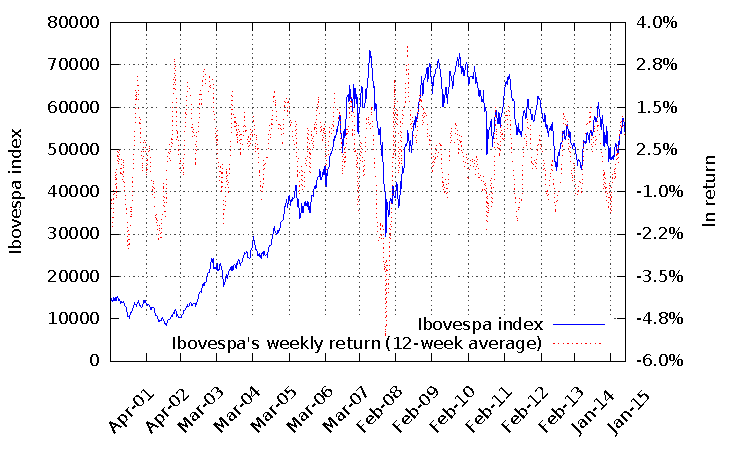
\includegraphics[width=5.5in,keepaspectratio]{ibov}
    \source{Author.}
    \label{fig:ibovespa}
\end{figure}

There are some possible approaches to define modes and their probability transition matrix. For instance, one could use econometric models, distributions adjustments as in \cite{doe0000}, or even simpler approaches without distribution adjustments as used in \cite{doe0000}.

We will follow a mixed but still similar methodology as suggested in \cite{smith0000} and \cite{smith0000}. The main difference of our methodology regards the the criteria to split the market return's distribution, keeping the focus on other technical aspects of the resulting operation modes.

Our approach consists by first defining three regions around the market's 12-week average return, $R_{avg}$, each with width of one standard deviation, $\sigma_R$, multiplied by an adjustment factor, $a_f$. Once we have the three middle regions with the same width, we will automatically be left with two regions at both extremes with no boundaries. Thus, each region will have the following interval:
%
\begin{itemize}
    \item Region 1: $]-\infty ,\quad R_{avg} - 1.5 a_f \sigma_R]$
    \item Region 2: $]R_{avg} - 1.5 a_f \sigma_R ,\quad R_{avg} - 0.5 a_f \sigma_R]$
    \item Region 3: $]R_{avg} - 0.5 a_f \sigma_R ,\quad R_{avg} + 0.5 a_f \sigma_R]$
    \item Region 4: $]R_{avg} + 0.5 a_f \sigma_R ,\quad R_{avg} + 1.5 a_f \sigma_R]$
    \item Region 5: $]R_{avg} + 1.5 a_f \sigma_R ,\quad +\infty[$
\end{itemize}

We then set the adjustment factor in order to obtain extremes regions with enough data points to be considered statistically significant as defined below. Thus, in our example, we proceeded with the Ibovespa's 12-week average returns distribution and defined each operation mode as described below.
%
\begin{description}
    \item[(i)] it shall have five operation modes considering scenarios of very low returns ("1 - Stress"), low returns ("2 - Low"), stable returns ("3 - Stable"), high returns ("4 - High"), and very high returns ("5 - Boom"); and
    \item[(ii)] every operation mode shall have more than 20 data points or at least 5\% of the total data points.
\end{description}

After computing the market's returns and their standard deviation, we set $a_f=1$ to obtain the intervals of each region as defined above. This led to 55 and 41 data points in the two extreme scenarios respectively, providing them enough data points to be statistically significant as defined in item (ii) above.

The distribution and the operation modes' intervals obtained are shown in Figure \ref{fig:ibov_dist} and Table \ref{tab:modes} below.
%
\begin{figure} [h!]
    \centering
    \caption{Ibovespa's operation modes distributions.}
    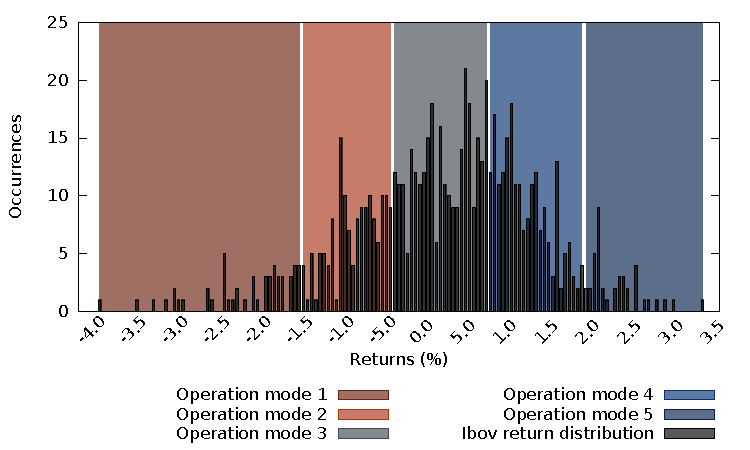
\includegraphics[width=6in,keepaspectratio]{distr}
    \source{Author.}
    \label{fig:ibov_dist}
\end{figure}
%
\begin{table}[h!]
    \caption{Market operation modes.}
    \centering
    \begin{tabular}{*{6}{c}}
        \specialrule{1.5pt}{2pt}{2pt}
        \multicolumn{2}{c}{} & \multicolumn{2}{c}{Returns' range} & \multicolumn{2}{c}{}                                      \\
        \specialrule{0.3pt}{2pt}{2pt}
        Mode                 & Description                        & $Min$                & $Max$     & Occurrence & Frequency \\
        \hline
        1                    & Stress                             & -$\infty$            & -1.5\%    & 55         & 7.4\%     \\
        2                    & Low                                & -1.5\%               & -0.4\%    & 158        & 21.4\%    \\
        3                    & Stable                             & -0.4\%               & 0.7\%     & 285        & 38.5\%    \\
        4                    & High                               & 0.7\%                & 1.9\%     & 201        & 27.2\%    \\
        5                    & Boom                               & 1.9\%                & +$\infty$ & 41         & 5.5\%     \\
        \specialrule{1.5pt}{2pt}{2pt}
    \end{tabular}
    \source{Author.}
    \label{tab:modes}
\end{table}

Once established the operation modes, we proceeded with the calculation of the  jumping frequencies to and from each mode.

The resulting transition probabilities is depicted in Table \ref{tab:transition}.
%
\begin{table}[h!]
    \caption{Operation modes transition matrix.}
    \centering
    \begin{tabular}{*{6}{c}}
        \specialrule{1.5pt}{2pt}{2pt}
             & \multicolumn{5}{c}{Mode}                                     \\
        \specialrule{0.3pt}{2pt}{2pt}
        Mode & 1                        & 2      & 3      & 4      & 5      \\
        \specialrule{0.3pt}{2pt}{2pt}
        1    & 70.9\%                   & 29.1\% & 0.0\%  & 0.0\%  & 0.0\%  \\
        2    & 9.5\%                    & 67.1\% & 23.4\% & 0.0\%  & 0.0\%  \\
        3    & 0.4\%                    & 12.0\% & 70.0\% & 16.9\% & 0.7\%  \\
        4    & 0.0\%                    & 0.5\%  & 23.8\% & 69.7\% & 6.0\%  \\
        5    & 0.0\%                    & 0.0\%  & 2.4\%  & 31.7\% & 65.9\% \\
        \specialrule{1.5pt}{2pt}{2pt}
    \end{tabular}
    \source{Author.}
    \label{tab:transition}
\end{table}

\subsection{Expected returns} \label{ss3}

In Table \ref{tab:returns} we show the annual average returns for each security given the operation modes obtained from the procedure described in the previous section.

Overall, the results followed the expected trend of higher returns for bullish markets and lower returns for bearish markets with the exception of the CDI asset in the Stress mode. There, the CDI provided a higher return probably due to a higher demand for safe assets and/or expectation that the fixed income benchmark rate would increase to tackle the potential money outflow from Brazil.
%
\begin{table}[h!]
    \caption{Annual expected returns per market operation mode.}
    \centering
    \begin{tabular}{*{6}{c}}
        \specialrule{1.5pt}{2pt}{2pt}
                 & \multicolumn{5}{c}{Mode}                                        \\
        \specialrule{0.3pt}{2pt}{2pt}
        Security & 1                        & 2       & 3      & 4       & 5       \\
        \specialrule{0.3pt}{2pt}{2pt}
        Ibov     & -68.6\%                  & -36.0\% & 10.7\% & 81.8\%  & 220.4\% \\
        CDI      & 14.6\%                   & 12.4\%  & 13.0\% & 13.9\%  & 18.8\%  \\
        EMBR3    & -49.8\%                  & -12.3\% & 9.9\%  & 21.2\%  & 188.3\% \\
        ITUB4    & -56.3\%                  & -26.1\% & 22.6\% & 86.5\%  & 143.3\% \\
        PETR4    & -70.3\%                  & -43.0\% & 16.1\% & 101.5\% & 136.5\% \\
        VALE5    & -53.5\%                  & -29.5\% & 23.5\% & 72.9\%  & 137.1\% \\
        \specialrule{1.5pt}{2pt}{2pt}
    \end{tabular}
    \source{Author.}
    \label{tab:returns}
\end{table}

\subsection{Expected covariances} \label{ss4}

The expected covariances were calculated using the same set of modes as described previously and their resulting upper triangular matrices are depicted in Tables \ref{tab:cov1}, \ref{tab:cov2}, \ref{tab:cov3}, \ref{tab:cov4}, and \ref{tab:cov5} below. Overall, we can notice that on average there is an increase in volatility from the Stable/High modes towards the Stress and Boom modes.
%
\begin{table}[h!]
    \caption{Annual expected covariances for mode 1.}
    \centering
    \begin{tabular}{*{7}{c}}
        \specialrule{1.5pt}{2pt}{2pt}
                 & \multicolumn{5}{c}{Security}                                                             \\
        \specialrule{0.3pt}{2pt}{2pt}
        Security & Ibov                         & CDI       & EMBR3     & ITUB4     & PETR4     & VALE5     \\
        \specialrule{0.3pt}{2pt}{2pt}
        Ibov     & 0.002609                     & -0.000006 & 0.002365  & 0.001177  & 0.002028  & 0.002984  \\
        CDI      &                              & 0.000016  & -0.000201 & 0.000016  & 0.000174  & 0.000264  \\
        EMBR3    &                              &           & 0.031981  & -0.000757 & -0.004895 & 0.001228  \\
        ITUB4    &                              &           &           & 0.003384  & 0.000300  & -0.000247 \\
        PETR4    &                              &           &           &           & 0.012779  & 0.007728  \\
        VALE5    &                              &           &           &           &           & 0.013388  \\
        \specialrule{1.5pt}{2pt}{2pt}
    \end{tabular}
    \source{Author.}
    \label{tab:cov1}
\end{table}
%
\begin{table}[h!]
    \caption{Annual expected covariances for mode 2.}
    \centering
    \begin{tabular}{*{7}{c}}
        \specialrule{1.5pt}{2pt}{2pt}
                 & \multicolumn{5}{c}{Security}                                                            \\
        \specialrule{0.3pt}{2pt}{2pt}
        Security & Ibov                         & CDI       & EMBR3     & ITUB4    & PETR4     & VALE5     \\
        \specialrule{0.3pt}{2pt}{2pt}
        Ibov     & 0.000444                     & -0.000007 & -0.000038 & 0.000432 & 0.000463  & 0.000116  \\
        CDI      &                              & 0.000024  & -0.000188 & 0.000002 & 0.000116  & 0.000128  \\
        EMBR3    &                              &           & 0.010090  & 0.000527 & -0.001179 & 0.000204  \\
        ITUB4    &                              &           &           & 0.002344 & 0.000159  & -0.000476 \\
        PETR4    &                              &           &           &          & 0.009060  & 0.002828  \\
        VALE5    &                              &           &           &          &           & 0.004521  \\
        \specialrule{1.5pt}{2pt}{2pt}
    \end{tabular}
    \source{Author.}
    \label{tab:cov2}
\end{table}
%
\begin{table}[h!]
    \caption{Annual expected covariances for mode 3.}
    \centering
    \begin{tabular}{*{7}{c}}
        \specialrule{1.5pt}{2pt}{2pt}
                 & \multicolumn{5}{c}{Security}                                                           \\
        \specialrule{0.3pt}{2pt}{2pt}
        Security & Ibov                         & CDI       & EMBR3     & ITUB4    & PETR4     & VALE5    \\
        \specialrule{0.3pt}{2pt}{2pt}
        Ibov     & 0.000549                     & -0.000001 & 0.000335  & 0.000684 & 0.000477  & 0.000506 \\
        CDI      &                              & 0.000030  & -0.000093 & 0.000053 & 0.000074  & 0.000065 \\
        EMBR3    &                              &           & 0.007809  & 0.000559 & -0.000724 & 0.000862 \\
        ITUB4    &                              &           &           & 0.002799 & 0.000296  & 0.000643 \\
        PETR4    &                              &           &           &          & 0.004692  & 0.000215 \\
        VALE5    &                              &           &           &          &           & 0.003980 \\
        \hline
    \end{tabular}
    \source{Author.}
    \label{tab:cov3}
\end{table}
%
\begin{table}[h!]
    \caption{Annual expected covariances for mode 4.}
    \centering
    \begin{tabular}{*{7}{c}}
        \specialrule{1.5pt}{2pt}{2pt}
                 & \multicolumn{5}{c}{Security}                                                          \\
        \specialrule{0.3pt}{2pt}{2pt}
        Security & Ibov                         & CDI      & EMBR3    & ITUB4    & PETR4     & VALE5     \\
        \specialrule{0.3pt}{2pt}{2pt}
        Ibov     & 0.000463                     & 0.000004 & 0.000339 & 0.000388 & 0.000484  & 0.000218  \\
        CDI      &                              & 0.000032 & 0.000115 & 0.000008 & -0.000015 & -0.000006 \\
        EMBR3    &                              &          & 0.007030 & 0.000209 & -0.000507 & -0.000134 \\
        ITUB4    &                              &          &          & 0.001542 & 0.000374  & -0.000042 \\
        PETR4    &                              &          &          &          & 0.004203  & 0.000030  \\
        VALE5    &                              &          &          &          &           & 0.005064  \\
        \specialrule{1.5pt}{2pt}{2pt}
    \end{tabular}
    \source{Author.}
    \label{tab:cov4}
\end{table}
%
\begin{table}[h!]
    \caption{Annual expected covariances for mode 5.}
    \centering
    \begin{tabular}{*{7}{c}}
        \specialrule{1.5pt}{2pt}{2pt}
                 & \multicolumn{5}{c}{Security}                                                             \\
        \specialrule{0.3pt}{2pt}{2pt}
        Security & Ibov                         & CDI       & EMBR3     & ITUB4     & PETR4     & VALE5     \\
        \specialrule{0.3pt}{2pt}{2pt}
        Ibov     & 0.000523                     & -0.000037 & 0.000444  & 0.000798  & 0.000460  & 0.000280  \\
        CDI      &                              & 0.000030  & -0.000132 & -0.000137 & -0.000085 & -0.000185 \\
        EMBR3    &                              &           & 0.010195  & -0.000587 & -0.002001 & -0.000020 \\
        ITUB4    &                              &           &           & 0.004025  & 0.002561  & 0.000753  \\
        PETR4    &                              &           &           &           & 0.005077  & 0.001845  \\
        VALE5    &                              &           &           &           &           & 0.006882  \\
        \specialrule{1.5pt}{2pt}{2pt}
    \end{tabular}
    \source{Author.}
    \label{tab:cov5}
\end{table}

\section{Simulations' results} \label{s2}

The objective in this section is to apply our results to a portfolio of financial securities, described by the System (\ref{eq:system}), and analyze its behavior when we impose a restriction on its total variance. We first simulate a portfolio under different levels of $\alpha$ and then we provide a sensitivity analysis for different risk parameters $\beta$ and $\nu$.

\subsection{Simulations for different levels of $\alpha$} \label{s_alpha}

The investments are allocated among one reference asset and four risky assets. The reference security will be the CDI and the risky assets will be EMBR3, ITUB4, PETR4, and VALE5.

We will use the parameters estimated previously to compute the matrices $\bar{A}$, $\tilde{A}$, $\bar{B}$, and $\tilde{B}$ as defined in Chapter \ref{chap:intro}. The matrix $\bar{A}$ represents the reference asset's return and $\bar{B}$ represents the risky assets' returns. The reference and risky assets' standard deviations matrices are associated with $\tilde{A}$ and $\tilde{B}$ respectively, where $\tilde{B}$ is obtained through the Cholesky decomposition of the covariance matrices.

Note that, while the matrices $\bar{A}$, $\tilde{A}$, $\bar{B}$, and $\tilde{B}$ are given in percentage terms, the system's output, $y(t)$, the portfolio's value, $x(k)$, and the control policy, $u(k)$, are all defined in monetary terms, $R\$$ in our case.

Our investment horizon is set at $T=20$ weeks and the initial wealth as $x(0) = 1$ monetary unity. The Markov chain will have $N=5$ operation modes starting at $\theta(0) = 3$ and its transition matrix is defined as in Table \ref{tab:transition}. The mutual correlation matrix between our multiplicative noises is defined as $\rho_{s1,s2}(k) = I$.

The weekly expected returns and standard deviations are then obtained through Tables \ref{tab:returns}, \ref{tab:cov1}, \ref{tab:cov2}, \ref{tab:cov3}, \ref{tab:cov4}, and \ref{tab:cov5} depending on the mode provided by the Markov chain on every $k=0, \cdots, T-1$.

We then define four scenarios to run our model according to Table \ref{tab:scenarios} below.
%
\begin{table}[h!]
    \caption{Scenarios definition.}
    \centering
    \begin{tabular}{*{6}{c}}
        \specialrule{1.5pt}{2pt}{2pt}
        \multicolumn{2}{c}{} & \multicolumn{3}{c}{Risk parameters}       & Restriction                                       \\
        \multicolumn{2}{c}{} & \multicolumn{3}{c}{$t = 1,2, \dotsc, 20$} & \textit{(R\$)}                                    \\
        \specialrule{0.3pt}{2pt}{2pt}
        Scenario             & Problem applied                           & $\nu(t)$       & $\xi(t)$ & $\beta(t)$ & $\alpha$ \\
        \specialrule{0.3pt}{2pt}{2pt}
        A                    & $PU(\nu,\xi)$                             & 1.0            & 1.0      & -          & -        \\
        B                    & $PC(\nu,\beta,\alpha)$                    & 1.0            & -        & 1.0        & 50.0     \\
        C                    & $PC(\nu,\beta,\alpha)$                    & 1.0            & -        & 1.0        & 20.0     \\
        D                    & $PC(\nu,\beta,\alpha)$                    & 1.0            & -        & 1.0        & 0.1      \\
        \specialrule{1.5pt}{2pt}{2pt}
    \end{tabular}
    \source{Author.}
    \label{tab:scenarios}
\end{table}

In the first scenario we solve the unconstrained problem, $PU(\nu,\xi)$, while in the other three scenarios we solve the $PC(\nu,\beta,\alpha)$ problem for different restrictions on the total variance, $\alpha$. In this way we can observe how the output, variance, and control policy change from an unconstrained problem to a constrained one with a decreasing total variance boundary.

The first scenario problem, $PU(\nu,\xi)$, is solved by following the steps as described in Section \ref{remark:uk}. %, Chapter \ref{chap:form}.

The $PC(\nu,\beta,\alpha)$ problem is solved following the same steps described in Section \ref{remark:uk}, however, we now take the restriction $\alpha$ into consideration by computing $\xi$ using Equation (\ref{tPC3:e1}) and $\beta$ as defined in Table \ref{tab:scenarios}. With this calculated $\xi$, we obtain $\lambda$ from Equation (\ref{PU:lambda}) and the optimal control policy of $PC(\nu,\beta,\alpha)$ using Equation (\ref{u_k}).

The risk parameters $\nu(t)$, $\xi(t)$, and  $\beta(t)$ were assumed to be equal to one in every time step. Thereby, by attributing the same risk relevance among all time steps related to both parameters, we are assuming that the investor has no risk bias towards neither the system's output nor its variance over time. Different risk aversion characteristics would lead to different relative weights among the elements of the risk parameters. In order to show how the results may change with changes in risk perceptions, we provided a sensitivity analysis for our $PC(\nu,\beta,\alpha)$ problem by changing $\beta$ and $\nu$ in Section \ref{specific} below.

Finally, after 10,000 simulations, we obtain the results shown in the following charts and Table \ref{tab:results}.
%
\begin{table}[h!]
    \caption{Resulting total variance and other parameters for $PC(\nu,\beta,\alpha)$ problem.}
    \centering
    \begin{tabular}{*{7}{c}}
        \specialrule{1.5pt}{2pt}{2pt}
        Scenario
          & $r_1$                             & $r_2$    & $r_3$ & $f(\beta,\alpha)$ & $\xi(t)$
          & $\sum_{t=1}^{T}\nu(t)Var[y^u(t)]$                                                           \\
        \specialrule{0.3pt}{2pt}{2pt}
        A & -                                 & -        & -     & -                 & 1.000    & 118.2 \\
        B & 118.2                             & -3.6e-15 & -50   & 0.651             & 0.651    & 50    \\
        C & 118.2                             & -3.6e-15 & -20   & 0.411             & 0.411    & 20    \\
        D & 118.2                             & -3.6e-15 & -0.1  & 0.029             & 0.029    & 0.1   \\
        \specialrule{1.5pt}{2pt}{2pt}
    \end{tabular}
    \source{Author.}
    \label{tab:results}
\end{table}

As expected, for all last three scenarios, the solution of $PC(\nu,\beta,\alpha)$ problem led to $\sum_{t=1}^{T}\nu(t)Var[y^u(t)] = \alpha$ by finding a proper $f(\beta,\alpha)$.

The output of the system is shown in Figure \ref{fig:output} below where we can see that an imposed lower total variance led to lower returns in every time step.
%
\begin{figure} [h!]
    \caption{System's output for all scenarios.}
    \centering
    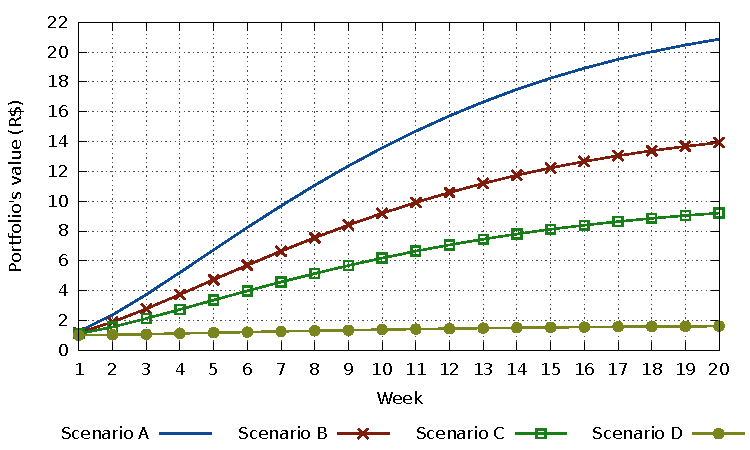
\includegraphics[width=6in,keepaspectratio]{y_t}
    \source{Author.}
    \label{fig:output}
\end{figure}

The variance over time for all scenarios is shown in Figure \ref{fig:var1}. In all cases we can see that the shape of the curve smooths gradually as the restriction $\alpha$ decreases, which means that although our restriction targets the total variance, we are able to lower the variance accordingly in each step providing that we have the same risk input parameters in each scenario.
%
\begin{figure} [h!]
    \caption{System's output variance for all scenarios.}
    \centering
    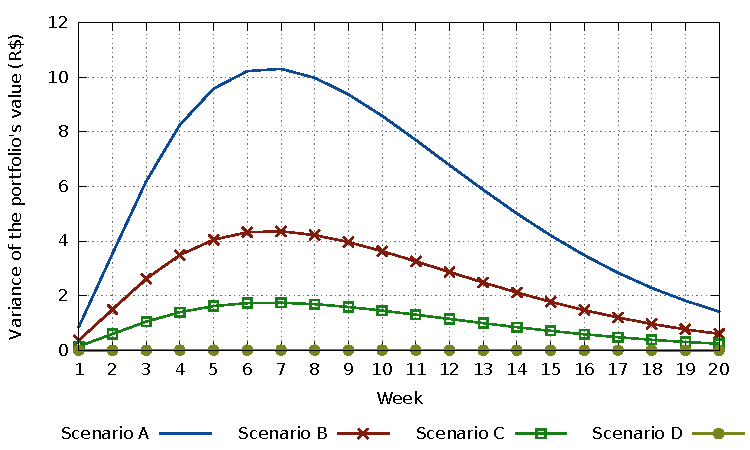
\includegraphics[width=6in,keepaspectratio]{var_1}
    \source{author.}
    \label{fig:var1}
\end{figure}

The control policies shown in Figures \ref{fig:u1}, \ref{fig:u2}, \ref{fig:u3}, and \ref{fig:u4} reveal that the introduction of a lower restriction on the variance forces the solution to distribute a lower volume in all risky assets while keeping almost the same relative allocation among them.

On the other hand, the lower volume in the risky assets is now counter-balanced by a reduction in the borrowings using the CDI. Notice that the CDI changes from an instrument of leverage to an investment in the later periods in scenario D, (Figure \ref{fig:u4}).

The results suggest that the proportional optimal allocation is barely affected by the total variance restriction and that the minimization of the total variance is done by managing the allocation in the risk-free asset.

In the limit, we will obtain a portfolio almost fully allocated in the CDI as our restriction $\alpha$ approaches zero. The only reason it does not reaches 100\% allocation in the CDI is because we have considered the correlations between the CDI and the other assets different than zero, which implies there will be no control policy for $\alpha=0$ in our example.

The numerical data analyzed in this chapter can be found in the appendix \ref{app:A}
%
\begin{figure} [H]
    \caption{Control policy for scenario A.}
    \centering
    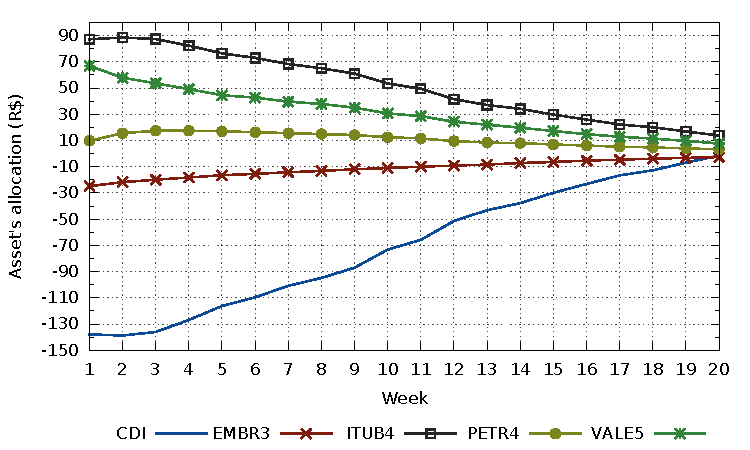
\includegraphics[width=6in,keepaspectratio]{u_A}
    \source{author.}
    \label{fig:u1}
\end{figure}
%
\begin{figure} [H]
    \caption{Control policy for scenario B.}
    \centering
    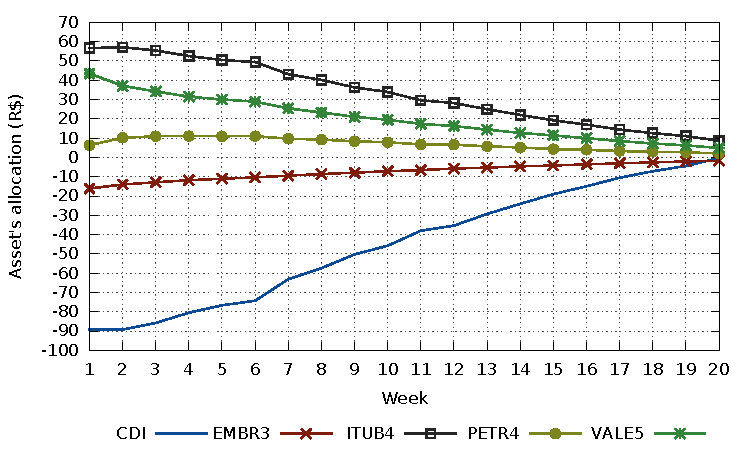
\includegraphics[width=6in,keepaspectratio]{u_B}
    \source{Author.}
    \label{fig:u2}
\end{figure}
%
\begin{figure} [H]
    \caption{Control policy for scenario C.}
    \centering
    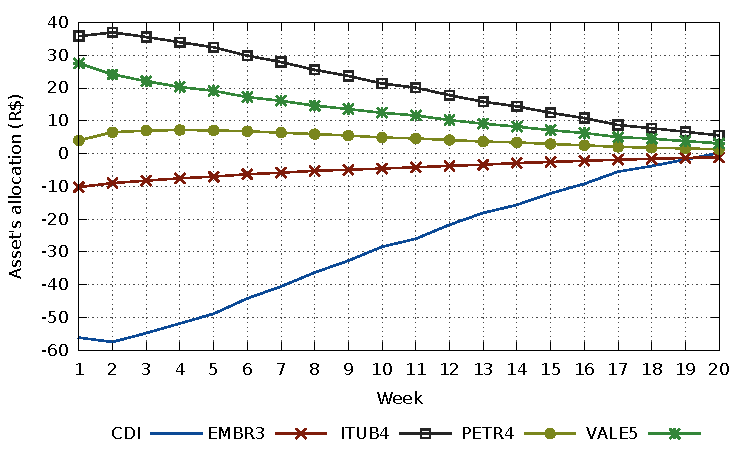
\includegraphics[width=6in,keepaspectratio]{u_C}
    \source{Author.}
    \label{fig:u3}
\end{figure}
%
\begin{figure} [H]
    \caption{Control policy for scenario D.}
    \centering
    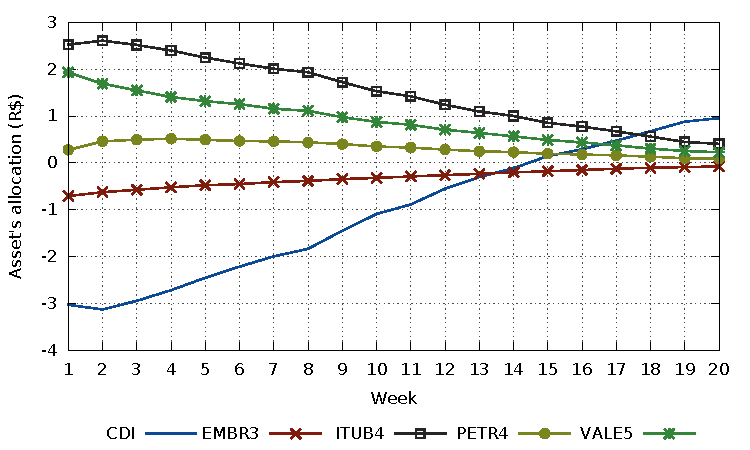
\includegraphics[width=6in,keepaspectratio]{u_D}
    \source{Author.}
    \label{fig:u4}
\end{figure}

\subsection{Sensitivity analysis for $\beta$ and $\nu$} \label{specific}

In the previous sections we described how to obtain the optimal allocation of assets in a portfolio using our results and also provided a sensitivity analysis regarding the restriction $\alpha$. Now, our goal is to illustrate how the portfolio's value, its variance and optimal assets allocation changes with variations in one single element of both risk parameters $\beta$ and $\nu$.

In this section, we simulate an arbitrary scenario where we say the investor wishes to increase the portfolio's value around step $t=t_a$ and decrease the portfolio's volatility around another step $t=t_b$, which is achieved by adjusting the values of $\beta(t_a)$ and $\nu(t_b)$, respectively. The other way around or any other combination of possible scenarios would lead to the same conclusions regarding the results' sensitivity and, therefore, were omitted in this analysis. Nonetheless, in the Appendix \ref{app:A}, we provide further sensitivity analysis for a diverse set of combinations of possible variations between the elements of $\beta$ and $\nu$ in order to illustrate the generalization of the conclusions laid out here and summarized in the next section.

The portfolio's assets and their characteristics are the same as described earlier in Section \ref{s1}. In order to facilitated the comparison among all scenarios, we will solve the $PC(\nu,\beta,\alpha)$ problem for the same arbitrary restriction, $\alpha=100$, in all scenarios and run  10,000 simulations to compute the results for each of them.

We start with a base scenario, $cc$, where the vectors $\beta$ and $\nu$ have all unitary elements and then we apply a variation in a single element of each vector to assess their effects on the portfolio's results. In order to ease the graphical observation of the variations in the results, we arbitrarily pick two specific time steps that are "sufficiently" distant from each other and, in this case, we chose $t_a=4$ and $t_b=9$. Then we set "big" enough new elements for $\beta(4)$ and $\nu(9)$ in order to get visible changes in our charts. After some try and error, we choose $\{3,5,7,9,11\}$ as the set of possible new coefficients' values for illustration purposes and label the following scenarios using the above rational, see Table \ref{tab:scenarios4}.
%
\begin{table}[h!]
    \caption{Scenarios that combine specific changes in the coefficients of $\beta$ and $\nu$ and a base scenario $cc$.}
    \centering
    \begin{tabular}{*{6}{c}}
        \specialrule{1.5pt}{2pt}{2pt}
        \multicolumn{2}{c}{} & \multicolumn{3}{c}{Input parameter}
                             & \multicolumn{1}{c}{}                                                                         \\
        \specialrule{0.3pt}{2pt}{2pt}
                             &                                     &            &            &          & Resulting         \\
        Scenario             & Problem applied                     & $\beta(4)$ & $\nu(9)$   & $\alpha$ & $f(\beta,\alpha)$ \\
        \specialrule{0.3pt}{2pt}{2pt}
        \textbf{cc}          & $PC(\nu,\beta,\alpha)$              & \textbf{1} & \textbf{1} & 100      & 0.920             \\
        \textbf{beta7}       & $PC(\nu,\beta,\alpha)$              & \textbf{7} & \textbf{1} & 100      & 0.819             \\
        \textbf{nu7}         & $PC(\nu,\beta,\alpha)$              & \textbf{1} & \textbf{7} & 100      & 1.050             \\
        \specialrule{0.3pt}{2pt}{2pt}
        COMBINED-3           & $PC(\nu,\beta,\alpha)$              & 3          & 3          & 100      & 0.939             \\
        COMBINED-5           & $PC(\nu,\beta,\alpha)$              & 5          & 5          & 100      & 0.937             \\
        \textbf{COMBINED-7}  & $PC(\nu,\beta,\alpha)$              & \textbf{7} & \textbf{7} & 100      & 0.925             \\
        COMBINED-9           & $PC(\nu,\beta,\alpha)$              & 9          & 9          & 100      & 0.907             \\
        COMBINED-11          & $PC(\nu,\beta,\alpha)$              & 11         & 11         & 100      & 0.887             \\
        \specialrule{1.5pt}{2pt}{2pt}
        \multicolumn{6}{c}{Note: $\beta(t)=1$ and $\nu(t)=1$ for all the remaining $t$, $t \in \{1,\cdots, 20\}-\{4,9\}$.}
    \end{tabular}
    \source{Author.}
    \label{tab:scenarios4}
\end{table}

We will focus the analysis based on four scenarios, $cc$, $beta7$, $nu7$, and $COMBINED-7$. This will allow us to see the specific effects around the scenario $cc$ by first changing $\beta(4)$ to $7$ in scenario $beta7$, by changing $\nu(9)$ to $7$ in scenario $nu7$, and then combining the effects of both changes in scenario $COMBINED-7$. The remaining scenarios will only be used to illustrated the sensitivity of the results of scenario $COMBINED-7$ for different levels of $\beta(4)$  and $\nu(9)$.

Figures \ref{fig:y_spec1} and \ref{fig:var_spec1} show the portfolio's value and its variance for the four scenarios described above. As one can easily observe in the curve of $beta7$ versus $cc$, an increase in $\beta(4)$ leads to an increase in the portfolio's value from $t=1$ up to $t=4$ followed by a correspondent increase in the variance. After $t=4$, $\beta$ decreases back to $1$ and the portfolio's value and its variance decreases.

In scenario $nu7$, we can see that an increase in $\nu(9)$ leads to a decrease in the variance from $t=3$ up to $t=9$ followed by a correspondent decrease in the portfolio's value. Then, at $t=10$, $\nu$ decreases back to 1 which leads to the opposite effect just described.


Note that, given we imposed a restriction on the total variance for all scenarios, $\alpha=100$, the higher variances obtained until $t=4$ in scenario $beta7$ will be compensated with lower variances in the later periods when compared with those from the base scenario $cc$. The same reasoning applies for scenario $nu7$, where the restriction $\alpha=100$ will force a compensation in the later periods leading them to show higher variances when compared with those from the base scenario $cc$. The correspondent returns in the later periods will follow their variances with the same trend of higher or lower values. However, the accumulated returns will also influence the final results and it explains why scenario $beta7$ showed a higher return than the one of scenario $nu7$ after $t=10$.

As we can see in scenario $COMBINED-7$, the combined effect of $\beta(4)=7$ and $\nu(9)=7$ leads to the same trends regarding the output and its variance as stated above. However, now there are some compensation on the final results due to the opposite effects of each variation.

Note that the parameters $\alpha=100$, $\beta(4)=7$, and $\nu(9)=7$ will affect all the values of the portfolio and their volatility over the whole time period, $T=20$. However, the strongest effect of $\beta(4)$ and $\nu(9)$ are around $t=4$ and $t=9$, respectively, which means that it is possible to be specific about the desired relevance of the portfolio's value and its volatility on each time step even though we can not be specific about the combined result a priori.

It is also worth to mention that by setting a coefficient seven times higher than any other coefficient does not mean achieving a portfolio's value seven times higher or a volatility seven times lower than otherwise.

In our example, the portfolio's value increased from around 5 to 6 by choosing $\beta(4)=7$, see curves $cc$ and $beta7$ in Figure \ref{fig:y_spec1} at $t=4$.
%
\begin{figure} [H]
    \caption{System's output for scenario $COMBINED-7$, $beta7$, $nu7$, and base scenario $cc$.}
    \centering
    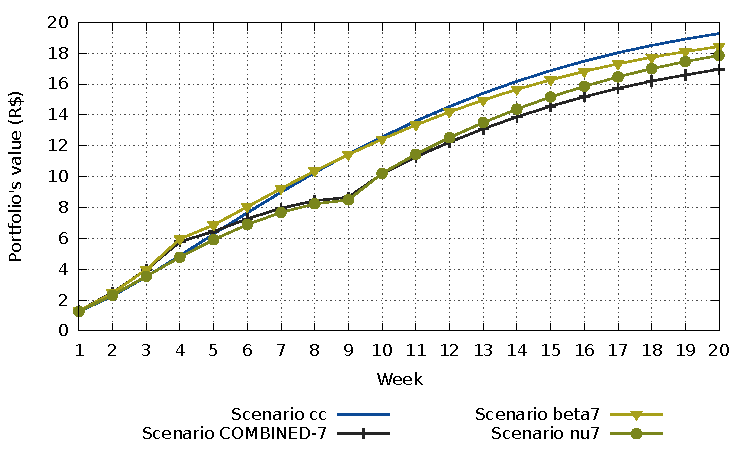
\includegraphics[width=5.9in,keepaspectratio]{y_spec1}
    \source{Author.}
    \label{fig:y_spec1}
\end{figure}
%
\begin{figure} [H]
    \caption{System's output variance for scenario $COMBINED-7$, $beta7$, $nu7$, and base scenario $cc$.}
    \centering
    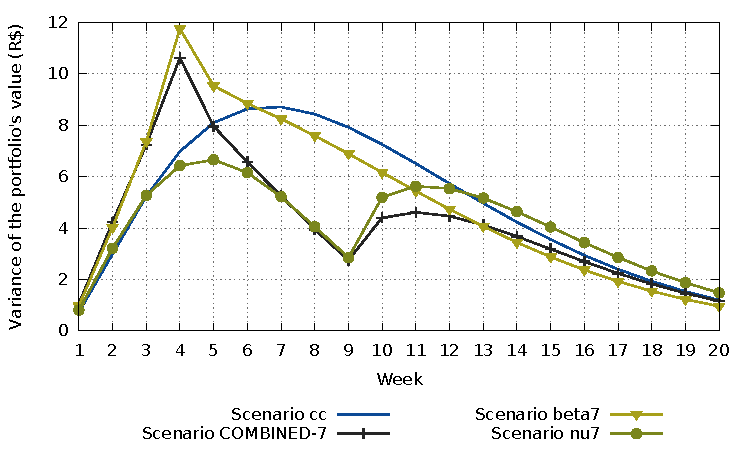
\includegraphics[width=5.9in,keepaspectratio]{var_spec1}
    \source{Author.}
    \label{fig:var_spec1}
\end{figure}

Looking at the wealth allocation for scenarios $COMBINED-7$ versus $cc$ in Figure \ref{fig:u_spec1}, we can see that setting a higher expected portfolio's value through  $\beta(4)=7$ leads to an increase in the wealth allocated in the risk assets and to a lower asset allocation in the risk-free asset up to $t=4$. In the same way, setting a lower volatility at $t=9$ through $\nu(9)=7$ forces the opposite effect on the wealth allocation.

Note that, after the point $t=9$, the asset allocation tends to the one of scenario $cc$ because the values $\beta(4)=7$ and $\nu(9)=7$ coincidentally counter-balanced each other in this short period of time. %in this example. However, this is not necessarily true if we choose other values for $\alpha$, $\beta(t)$, and $\nu(t)$.
%
\begin{figure} [H]
    \caption{Control policy for scenario $COMBINED-7$ versus the base scenario $cc$.}
    \centering
    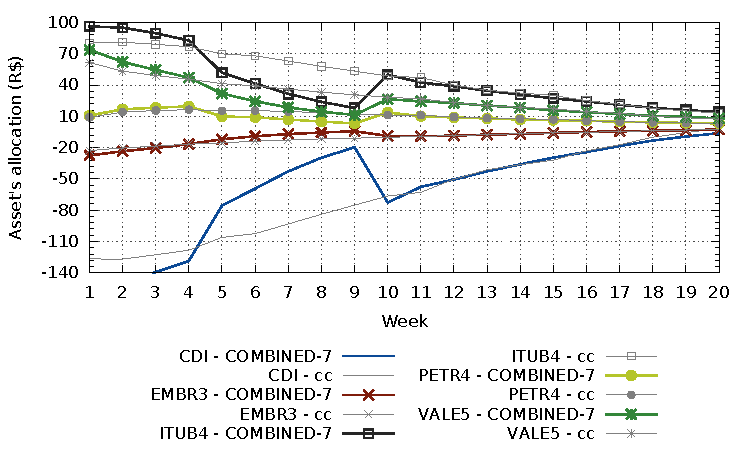
\includegraphics[width=6in,keepaspectratio]{u_spec1}
    \source{Author.}
    \label{fig:u_spec1}
\end{figure}

The results for the remaining scenarios of Table \ref{tab:scenarios4} will lead to an identical conclusion to the one described above and, therefore, we will only show their results in Figures \ref{fig:y_spec56789} and \ref{fig:var_spec56789} to illustrate the sensitivity of the output and the variance around scenario $cc$ for different values of $\beta(4)$ and $\nu(9)$.

Note that the variations in the portfolio's value and in its variance are not proportional to the changes in the coefficients, illustrating our comments above.
%
\begin{figure} [H]
    \caption{System's output for scenario $COMBINED-5,6,7,8,9$ and base scenario $cc$.}
    \centering
    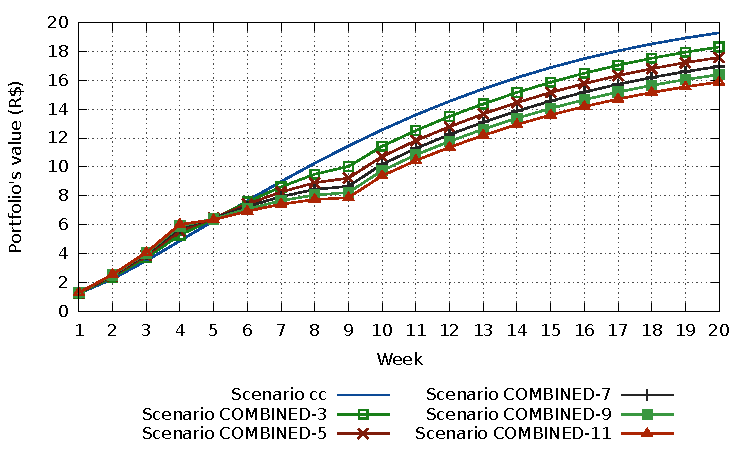
\includegraphics[width=6in,keepaspectratio]{y_spec56789}
    \source{Author.}
    \label{fig:y_spec56789}
\end{figure}
%
\begin{figure} [H]
    \caption{System's output variance for scenario $COMBINED-5,6,7,8,9$ and base scenario $cc$.}
    \centering
    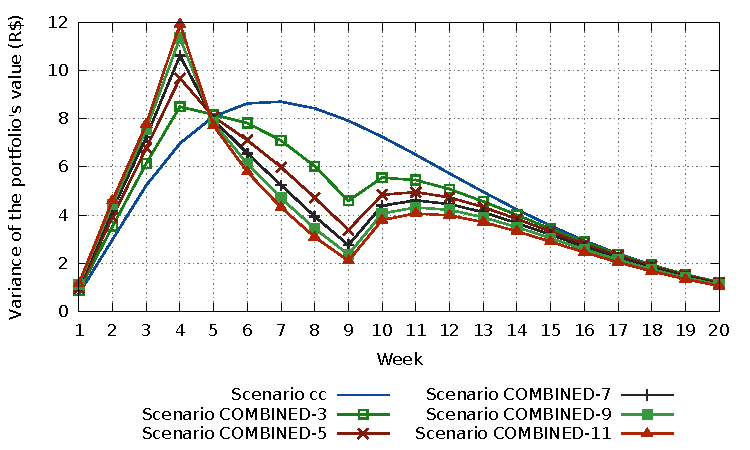
\includegraphics[width=6in,keepaspectratio]{var_spec56789}
    \source{Author.}
    \label{fig:var_spec56789}
\end{figure}
\vfill

\subsection{Sensitivity analysis summary and final comments} \label{sens_summary}

Following the above discussion and recalling the effects of $\alpha$ from the analysis carried out in Section \ref{s_alpha}, we can summarize the effects that $\beta$, $\nu$, and $\alpha$ will have on the expected system's output, its variance, and on the wealth allocation policy, see Table \ref{tab:summary}.
%
\begin{table}[h!]
    \caption{Effects of changes in $\beta$, $\nu$, and $\alpha$ on the expected portfolio's value, its variance, and on the wealth allocation policy.}
    \centering
    \begin{tabular}{*{5}{c}}
        \specialrule{1.5pt}{2pt}{2pt}
        \multicolumn{3}{c}{}    & \multicolumn{2}{c}{Wealth allocation on}                                                 \\
        \specialrule{0.3pt}{2pt}{2pt}
        Risk parameter          & $E[y^u(t)]$                              & $Var[y^u(t)]$ & risk assets & risk-free asset \\
        \specialrule{0.3pt}{2pt}{2pt}
        $\beta(t)$ $\uparrow$   & $\uparrow$                               & $\uparrow$
                                & $\uparrow$                               & $\downarrow$                                  \\
        $\beta(t)$ $\downarrow$ & $\downarrow$                             & $\downarrow$
                                & $\downarrow$                             & $\uparrow$                                    \\
        $\nu(t)$ $\uparrow$     & $\downarrow$                             & $\downarrow$
                                & $\downarrow$                             & $\uparrow$                                    \\
        $\nu(t)$ $\downarrow$   & $\uparrow$                               & $\uparrow$
                                & $\uparrow$                               & $\downarrow$                                  \\
        $\alpha$ $\uparrow$     & $\uparrow$                               & $\uparrow$
                                & $\uparrow$                               & $\downarrow$                                  \\
        $\alpha$ $\downarrow$   & $\downarrow$                             & $\downarrow$
                                & $\downarrow$                             & $\uparrow$                                    \\
        \specialrule{1.5pt}{2pt}{2pt}
    \end{tabular}
    \source{Author.}
    \label{tab:summary}
\end{table}

Note that these general effects are valid for variations within the elements of $\beta$ and $\nu$ as well as variations between the cross elements of those vectors.

Nonetheless, there is no standard or scientific procedure to determine the exactly coefficients that someone should use as inputs for our risk parameters. In order to understand and recognize the investor's risk-aversion/risk-taking sentiment and the trade-offs between $\beta$, $\nu$, and $\alpha$, we suggest a similar analysis to the one developed in this chapter, where through modeling and testing different scenarios, someone would be able to understand the potential gains and losses involved and what would be the proper parameters inputs that represent his/her boundary conditions regarding returns and variances over time.

\vfill


\chapter{Conclusion} \label{chap:conclusion}

In this work we have considered ...


Post-textual elements
\bibliography{doc/bibliography}
\appendix
\chapter{Numerical data of simulations} \label{app:A}

Example of long tables that cross pages.

\setstretch{1.3}

\begin{center}
\begin{longtable}{*{5}{c}}
	\caption{System's output for all scenarios.}\\
	\specialrule{1.5pt}{2pt}{2pt}
	Time	& Scenario 1	& Scenario 2	& Scenario 3	& Scenario 4 \\
	\specialrule{0.1pt}{2pt}{2pt}
	\endfirsthead

	\specialrule{1.5pt}{2pt}{2pt}
	Time	& Scenario 1	& Scenario 2	& Scenario 3	& Scenario 4 \\
	\specialrule{0.1pt}{2pt}{2pt}
	\endhead

	\specialrule{0.3pt}{2pt}{2pt}
	\multicolumn{5}{c}{{Continued on next page}} \\
	\specialrule{0.3pt}{2pt}{2pt}
	\endfoot
	\endlastfoot

		1	& 1.3	& 1.2	& 1.1	& 1.0\\
		2	& 2.4	& 1.9	& 1.6	& 1.0\\
		3	& 3.7	& 2.8	& 2.1	& 1.1\\
		4	& 5.2	& 3.7	& 2.7	& 1.2\\
		5	& 6.7	& 4.7	& 3.4	& 1.2\\
		6	& 8.2	& 5.7	& 4.0	& 1.3\\
		7	& 9.7	& 6.7	& 4.6	& 1.3\\
		8	& 11.1	& 7.6	& 5.2	& 1.4\\
		9	& 12.4	& 8.4	& 5.7	& 1.4\\
		10	& 13.6	& 9.2	& 6.2	& 1.4\\
		11	& 14.7	& 9.9	& 6.7	& 1.5\\
		12	& 15.7	& 10.6	& 7.1	& 1.5\\
		13	& 16.7	& 11.2	& 7.5	& 1.5\\
		14	& 17.5	& 11.7	& 7.8	& 1.5\\
		15	& 18.3	& 12.2	& 8.1	& 1.6\\
		16	& 18.9	& 12.7	& 8.4	& 1.6\\
		17	& 19.5	& 13.1	& 8.6	& 1.6\\
		18	& 20.0	& 13.4	& 8.9	& 1.6\\
		19	& 20.5	& 13.7	& 9.0	& 1.6\\
		20	& 20.9	& 13.9	& 9.2	& 1.6\\
		\specialrule{0.3pt}{2pt}{2pt}
		\multicolumn{5}{c}{Source: Author.}
\end{longtable}

%
\begin{longtable}{*{5}{c}}
	\caption{System's output variance for all scenarios.}\\
	\specialrule{1.5pt}{2pt}{2pt}
	Time	& Scenario 1	& Scenario 2	& Scenario 3	& Scenario 4 \\
	\specialrule{0.1pt}{2pt}{2pt}
	\endfirsthead

	\specialrule{1.5pt}{2pt}{2pt}
	Time	& Scenario 1	& Scenario 2	& Scenario 3	& Scenario 4 \\
	\specialrule{0.1pt}{2pt}{2pt}
	\endhead

	\specialrule{0.3pt}{2pt}{2pt}
	\multicolumn{5}{c}{{Continued on next page}} \\
	\specialrule{0.3pt}{2pt}{2pt}
	\endfoot
	\endlastfoot
		1	& 0.86	& 0.37	& 0.15	& 0.0007\\
		2	& 3.54	& 1.50	& 0.60	& 0.003\\
		3	& 6.19	& 2.62	& 1.05	& 0.005\\
		4	& 8.25	& 3.49	& 1.40	& 0.007\\
		5	& 9.58	& 4.05	& 1.62	& 0.008\\
		6	& 10.21	& 4.32	& 1.73	& 0.009\\
		7	& 10.30	& 4.36	& 1.74	& 0.009\\
		8	& 9.97	& 4.22	& 1.69	& 0.008\\
		9	& 9.37	& 3.96	& 1.58	& 0.008\\
		10	& 8.58	& 3.63	& 1.45	& 0.007\\
		11	& 7.70	& 3.25	& 1.30	& 0.007\\
		12	& 6.78	& 2.87	& 1.15	& 0.006\\
		13	& 5.87	& 2.48	& 0.99	& 0.005\\
		14	& 5.01	& 2.12	& 0.85	& 0.004\\
		15	& 4.20	& 1.78	& 0.71	& 0.004\\
		16	& 3.48	& 1.47	& 0.59	& 0.003\\
		17	& 2.84	& 1.20	& 0.48	& 0.002\\
		18	& 2.28	& 0.97	& 0.39	& 0.002\\
		19	& 1.81	& 0.77	& 0.31	& 0.002\\
		20	& 1.42	& 0.60	& 0.24	& 0.001\\
		\specialrule{0.3pt}{2pt}{2pt}
		\multicolumn{5}{c}{Source: Author.}
\end{longtable}

%
\begin{longtable}{*{6}{c}}
	\caption{Control policy for scenario A.}\\
	\specialrule{1.5pt}{2pt}{2pt}
	Time	& CDI	& EMBR3	& ITUB4	& PETR4	& VALE5 \\
	\specialrule{0.1pt}{2pt}{2pt}
	\endfirsthead

	\specialrule{1.5pt}{2pt}{2pt}
	Time	& CDI	& EMBR3	& ITUB4	& PETR4	& VALE5 \\
	\specialrule{0.1pt}{2pt}{2pt}
	\endhead

	\specialrule{0.3pt}{2pt}{2pt}
	\multicolumn{6}{c}{{Continued on next page}} \\
	\specialrule{0.3pt}{2pt}{2pt}
	\endfoot
	\endlastfoot

		0	& -137.9	& -24.9	& 87.1	& 9.8	& 66.9\\
		1	& -138.7	& -21.8	& 88.5	& 15.5	& 57.8\\
		2	& -136.0	& -20.0	& 87.3	& 17.4	& 53.6\\
		3	& -126.9	& -18.2	& 82.3	& 17.4	& 49.1\\
		4	& -116.2	& -16.5	& 76.4	& 17.0	& 44.5\\
		5	& -109.6	& -15.5	& 72.9	& 16.3	& 42.6\\
		6	& -100.9	& -14.3	& 68.3	& 15.6	& 39.6\\
		7	& -94.8		& -13.3	& 65.1	& 14.8	& 37.8\\
		8	& -87.0		& -12.0	& 60.9	& 14.2	& 35.0\\
		9	& -73.2		& -11.0	& 53.5	& 12.5	& 30.6\\
		10	& -65.9		& -10.0	& 49.4	& 11.5	& 28.5\\
		11	& -51.4		& -9.2	& 41.5	& 9.6	& 24.2\\
		12	& -43.2		& -8.4	& 37.0	& 8.3	& 22.0\\
		13	& -37.8		& -7.2	& 34.1	& 7.9	& 19.7\\
		14	& -29.9		& -6.4	& 29.7	& 6.9	& 17.2\\
		15	& -23.2		& -5.4	& 25.9	& 6.1	& 14.8\\
		16	& -16.6		& -4.6	& 22.2	& 5.2	& 12.8\\
		17	& -12.7		& -3.9	& 20.0	& 4.7	& 11.4\\
		18	& -7.0		& -3.3	& 16.8	& 3.9	& 9.7\\
		19	& -1.6		& -2.7	& 13.7	& 3.3	& 7.7\\
		\specialrule{0.3pt}{2pt}{2pt}
		\multicolumn{6}{c}{Source: Author.}
\end{longtable}

%
\begin{longtable}{*{6}{c}}
	\caption{Control policy for scenario B.}\\
	\specialrule{1.5pt}{2pt}{2pt}
	Time	& CDI	& EMBR3	& ITUB4	& PETR4	& VALE5 \\
	\specialrule{0.1pt}{2pt}{2pt}
	\endfirsthead

	\specialrule{1.5pt}{2pt}{2pt}
	Time	& CDI	& EMBR3	& ITUB4	& PETR4	& VALE5 \\
	\specialrule{0.1pt}{2pt}{2pt}
	\endhead

	\specialrule{0.3pt}{2pt}{2pt}
	\multicolumn{6}{c}{{Continued on next page}} \\
	\specialrule{0.3pt}{2pt}{2pt}
	\endfoot
	\endlastfoot

		0	& -89.3		& -16.2	& 56.6	& 6.4	& 43.5\\
		1	& -89.3		& -14.0	& 57.2	& 10.2	& 37.1\\
		2	& -85.8		& -12.9	& 55.4	& 11.0	& 34.2\\
		3	& -80.5		& -11.8	& 52.6	& 11.1	& 31.5\\
		4	& -76.7		& -11.1	& 50.5	& 11.0	& 30.0\\
		5	& -74.3		& -10.3	& 49.4	& 11.0	& 28.9\\
		6	& -63.1		& -9.4	& 43.2	& 9.7	& 25.4\\
		7	& -57.4		& -8.6	& 40.2	& 9.2	& 23.3\\
		8	& -50.3		& -7.9	& 36.3	& 8.4	& 21.1\\
		9	& -45.8		& -7.2	& 33.9	& 7.9	& 19.5\\
		10	& -38.0		& -6.6	& 29.6	& 6.7	& 17.4\\
		11	& -35.3		& -5.8	& 28.2	& 6.6	& 16.3\\
		12	& -29.3		& -5.3	& 25.0	& 5.8	& 14.4\\
		13	& -24.1		& -4.6	& 22.0	& 5.2	& 12.7\\
		14	& -19.0		& -4.2	& 19.2	& 4.3	& 11.4\\
		15	& -14.9		& -3.6	& 17.0	& 3.9	& 9.9\\
		16	& -10.5		& -3.1	& 14.4	& 3.3	& 8.5\\
		17	& -7.1		& -2.6	& 12.6	& 3.0	& 7.2\\
		18	& -4.4		& -2.1	& 11.0	& 2.6	& 6.2\\
		19	& -0.3		& -1.7	& 8.7	& 2.1	& 4.9\\
		\specialrule{0.3pt}{2pt}{2pt}
		\multicolumn{6}{c}{Source: Author.}
\end{longtable}

\end{center}

\vfill
\setstretch{\doubleSpacingRate}

\annex
\chapter{Numerical data of simulations} \label{an:A}

Example of long tables that cross pages.

\setstretch{1.3}

\begin{center}
\begin{longtable}{*{5}{c}}
	\caption{System's output for all scenarios.}\\
	\specialrule{1.5pt}{2pt}{2pt}
	Time	& Scenario 1	& Scenario 2	& Scenario 3	& Scenario 4 \\
	\specialrule{0.1pt}{2pt}{2pt}
	\endfirsthead

	\specialrule{1.5pt}{2pt}{2pt}
	Time	& Scenario 1	& Scenario 2	& Scenario 3	& Scenario 4 \\
	\specialrule{0.1pt}{2pt}{2pt}
	\endhead

	\specialrule{0.3pt}{2pt}{2pt}
	\multicolumn{5}{c}{{Continued on next page}} \\
	\specialrule{0.3pt}{2pt}{2pt}
	\endfoot
	\endlastfoot

		1	& 1.3	& 1.2	& 1.1	& 1.0\\
		2	& 2.4	& 1.9	& 1.6	& 1.0\\
		3	& 3.7	& 2.8	& 2.1	& 1.1\\
		4	& 5.2	& 3.7	& 2.7	& 1.2\\
		5	& 6.7	& 4.7	& 3.4	& 1.2\\
		6	& 8.2	& 5.7	& 4.0	& 1.3\\
		7	& 9.7	& 6.7	& 4.6	& 1.3\\
		8	& 11.1	& 7.6	& 5.2	& 1.4\\
		9	& 12.4	& 8.4	& 5.7	& 1.4\\
		10	& 13.6	& 9.2	& 6.2	& 1.4\\
		11	& 14.7	& 9.9	& 6.7	& 1.5\\
		12	& 15.7	& 10.6	& 7.1	& 1.5\\
		13	& 16.7	& 11.2	& 7.5	& 1.5\\
		14	& 17.5	& 11.7	& 7.8	& 1.5\\
		15	& 18.3	& 12.2	& 8.1	& 1.6\\
		16	& 18.9	& 12.7	& 8.4	& 1.6\\
		17	& 19.5	& 13.1	& 8.6	& 1.6\\
		18	& 20.0	& 13.4	& 8.9	& 1.6\\
		19	& 20.5	& 13.7	& 9.0	& 1.6\\
		20	& 20.9	& 13.9	& 9.2	& 1.6\\
		\specialrule{0.3pt}{2pt}{2pt}
		\multicolumn{5}{c}{Source: Author.}
\end{longtable}

%
\begin{longtable}{*{5}{c}}
	\caption{System's output variance for all scenarios.}\\
	\specialrule{1.5pt}{2pt}{2pt}
	Time	& Scenario 1	& Scenario 2	& Scenario 3	& Scenario 4 \\
	\specialrule{0.1pt}{2pt}{2pt}
	\endfirsthead

	\specialrule{1.5pt}{2pt}{2pt}
	Time	& Scenario 1	& Scenario 2	& Scenario 3	& Scenario 4 \\
	\specialrule{0.1pt}{2pt}{2pt}
	\endhead

	\specialrule{0.3pt}{2pt}{2pt}
	\multicolumn{5}{c}{{Continued on next page}} \\
	\specialrule{0.3pt}{2pt}{2pt}
	\endfoot
	\endlastfoot
		1	& 0.86	& 0.37	& 0.15	& 0.0007\\
		2	& 3.54	& 1.50	& 0.60	& 0.003\\
		3	& 6.19	& 2.62	& 1.05	& 0.005\\
		4	& 8.25	& 3.49	& 1.40	& 0.007\\
		5	& 9.58	& 4.05	& 1.62	& 0.008\\
		6	& 10.21	& 4.32	& 1.73	& 0.009\\
		7	& 10.30	& 4.36	& 1.74	& 0.009\\
		8	& 9.97	& 4.22	& 1.69	& 0.008\\
		9	& 9.37	& 3.96	& 1.58	& 0.008\\
		10	& 8.58	& 3.63	& 1.45	& 0.007\\
		11	& 7.70	& 3.25	& 1.30	& 0.007\\
		12	& 6.78	& 2.87	& 1.15	& 0.006\\
		13	& 5.87	& 2.48	& 0.99	& 0.005\\
		14	& 5.01	& 2.12	& 0.85	& 0.004\\
		15	& 4.20	& 1.78	& 0.71	& 0.004\\
		16	& 3.48	& 1.47	& 0.59	& 0.003\\
		17	& 2.84	& 1.20	& 0.48	& 0.002\\
		18	& 2.28	& 0.97	& 0.39	& 0.002\\
		19	& 1.81	& 0.77	& 0.31	& 0.002\\
		20	& 1.42	& 0.60	& 0.24	& 0.001\\
		\specialrule{0.3pt}{2pt}{2pt}
		\multicolumn{5}{c}{Source: Author.}
\end{longtable}

%
\begin{longtable}{*{6}{c}}
	\caption{Control policy for scenario A.}\\
	\specialrule{1.5pt}{2pt}{2pt}
	Time	& CDI	& EMBR3	& ITUB4	& PETR4	& VALE5 \\
	\specialrule{0.1pt}{2pt}{2pt}
	\endfirsthead

	\specialrule{1.5pt}{2pt}{2pt}
	Time	& CDI	& EMBR3	& ITUB4	& PETR4	& VALE5 \\
	\specialrule{0.1pt}{2pt}{2pt}
	\endhead

	\specialrule{0.3pt}{2pt}{2pt}
	\multicolumn{6}{c}{{Continued on next page}} \\
	\specialrule{0.3pt}{2pt}{2pt}
	\endfoot
	\endlastfoot

		0	& -137.9	& -24.9	& 87.1	& 9.8	& 66.9\\
		1	& -138.7	& -21.8	& 88.5	& 15.5	& 57.8\\
		2	& -136.0	& -20.0	& 87.3	& 17.4	& 53.6\\
		3	& -126.9	& -18.2	& 82.3	& 17.4	& 49.1\\
		4	& -116.2	& -16.5	& 76.4	& 17.0	& 44.5\\
		5	& -109.6	& -15.5	& 72.9	& 16.3	& 42.6\\
		6	& -100.9	& -14.3	& 68.3	& 15.6	& 39.6\\
		7	& -94.8		& -13.3	& 65.1	& 14.8	& 37.8\\
		8	& -87.0		& -12.0	& 60.9	& 14.2	& 35.0\\
		9	& -73.2		& -11.0	& 53.5	& 12.5	& 30.6\\
		10	& -65.9		& -10.0	& 49.4	& 11.5	& 28.5\\
		11	& -51.4		& -9.2	& 41.5	& 9.6	& 24.2\\
		12	& -43.2		& -8.4	& 37.0	& 8.3	& 22.0\\
		13	& -37.8		& -7.2	& 34.1	& 7.9	& 19.7\\
		14	& -29.9		& -6.4	& 29.7	& 6.9	& 17.2\\
		15	& -23.2		& -5.4	& 25.9	& 6.1	& 14.8\\
		16	& -16.6		& -4.6	& 22.2	& 5.2	& 12.8\\
		17	& -12.7		& -3.9	& 20.0	& 4.7	& 11.4\\
		18	& -7.0		& -3.3	& 16.8	& 3.9	& 9.7\\
		19	& -1.6		& -2.7	& 13.7	& 3.3	& 7.7\\
		\specialrule{0.3pt}{2pt}{2pt}
		\multicolumn{6}{c}{Source: Author.}
\end{longtable}

%
\begin{longtable}{*{6}{c}}
	\caption{Control policy for scenario B.}\\
	\specialrule{1.5pt}{2pt}{2pt}
	Time	& CDI	& EMBR3	& ITUB4	& PETR4	& VALE5 \\
	\specialrule{0.1pt}{2pt}{2pt}
	\endfirsthead

	\specialrule{1.5pt}{2pt}{2pt}
	Time	& CDI	& EMBR3	& ITUB4	& PETR4	& VALE5 \\
	\specialrule{0.1pt}{2pt}{2pt}
	\endhead

	\specialrule{0.3pt}{2pt}{2pt}
	\multicolumn{6}{c}{{Continued on next page}} \\
	\specialrule{0.3pt}{2pt}{2pt}
	\endfoot
	\endlastfoot

		0	& -89.3		& -16.2	& 56.6	& 6.4	& 43.5\\
		1	& -89.3		& -14.0	& 57.2	& 10.2	& 37.1\\
		2	& -85.8		& -12.9	& 55.4	& 11.0	& 34.2\\
		3	& -80.5		& -11.8	& 52.6	& 11.1	& 31.5\\
		4	& -76.7		& -11.1	& 50.5	& 11.0	& 30.0\\
		5	& -74.3		& -10.3	& 49.4	& 11.0	& 28.9\\
		6	& -63.1		& -9.4	& 43.2	& 9.7	& 25.4\\
		7	& -57.4		& -8.6	& 40.2	& 9.2	& 23.3\\
		8	& -50.3		& -7.9	& 36.3	& 8.4	& 21.1\\
		9	& -45.8		& -7.2	& 33.9	& 7.9	& 19.5\\
		10	& -38.0		& -6.6	& 29.6	& 6.7	& 17.4\\
		11	& -35.3		& -5.8	& 28.2	& 6.6	& 16.3\\
		12	& -29.3		& -5.3	& 25.0	& 5.8	& 14.4\\
		13	& -24.1		& -4.6	& 22.0	& 5.2	& 12.7\\
		14	& -19.0		& -4.2	& 19.2	& 4.3	& 11.4\\
		15	& -14.9		& -3.6	& 17.0	& 3.9	& 9.9\\
		16	& -10.5		& -3.1	& 14.4	& 3.3	& 8.5\\
		17	& -7.1		& -2.6	& 12.6	& 3.0	& 7.2\\
		18	& -4.4		& -2.1	& 11.0	& 2.6	& 6.2\\
		19	& -0.3		& -1.7	& 8.7	& 2.1	& 4.9\\
		\specialrule{0.3pt}{2pt}{2pt}
		\multicolumn{6}{c}{Source: Author.}
\end{longtable}

\end{center}

\vfill
\setstretch{\doubleSpacingRate}

\end{document}
